\documentclass[oneside, mag]{mgr}	
 
\usepackage{polski}	
\usepackage[utf8]{inputenc}	
\usepackage{amsmath}		
\usepackage{graphicx}	
\graphicspath{ {./} }
\usepackage{amsfonts}
\usepackage{hyperref}
\usepackage{tabstackengine}
\usepackage{caption}
\usepackage{subfig}
\usepackage{listings}
\usepackage[ruled,vlined]{algorithm2e}
\usepackage{tikz}
\usetikzlibrary{positioning} 
\usepackage{array}
\usepackage{makecell}
%test
\usepackage{multirow}
\usepackage{rotating}
\usepackage{gensymb}

\usepackage{mwe}

\renewcommand\theadalign{bc}
\renewcommand\theadfont{\bfseries}
\renewcommand\theadgape{\Gape[4pt]}
\renewcommand\cellgape{\Gape[4pt]}

\newcommand{\bb}{\textbf}

\newcommand{\specialcell}[2][c]{%
  \begin{tabular}[#1]{@{}c@{}}#2\end{tabular}}

\title{Analiza efektywności zastosowania sieci rekurencyjnych w zadaniu klasyfikacji}	
\engtitle{Analysis of the effectiveness of recursive networks in the classification task}
\author{Jędrzej Kozal}
\supervisor{dr  inż. Paweł Ksieniewicz}

\field{Informatyka (Inf)}
\specialisation{Systemy informatyki w medycynie (IMT)}

\begin{document}
\bibliographystyle{plabbrv}	

\maketitle

\section*{Podziękowania}

Chciałbym podziękować Michałowi Lesiowi za udostępnienie nakładów mocy obliczeniowej niezbędnej do przeprowadzenia badań, oraz za jego cierpliwość i wyrozumiałość, bez których ta praca by nie powstała.

\setcounter{tocdepth}{1}
\tableofcontents

\newpage
%\begin{flushright}
%Pracę chciałbym dedykować mojej babci Leokadii, \\ za jej %dyscyplinę, zorganizowanie i ciekawość świata. 
%\end{flushright}
%\newpage

%Wykaz skrótów:\\
%RNN - rekurencyjna sieć neuronowa (recurrent neural network)\\
%BPTT - propagacja wsteczna w czasie (back-propgation through time)\\
%LSTM - Long Short-Term Memory \\
%GRU - Gated Reccurent Unit \\

%Wykaz symboli matematycznych: \\
%$\odot$ - iloczyn Hadamarda \\
%\newpage

\chapter{Wstęp}

W niniejszym rozdziale zarysowano problematykę pracy i pokrótce omówiono zagadnienia, które będą wykorzystywane w dalszej części. Dokonano przeglądu literaturowego i opisano plan badań.

\section{Wprowadzenie}

Sekcja ta zawiera wprowadzenie podstawowych zagadnień, wykorzystywanych w pracy, oraz nakreślona rys historyczny badań związanych z tematyką pracy.

\subsection{Sieci neuronowe}

\begin{figure}
	\centering
	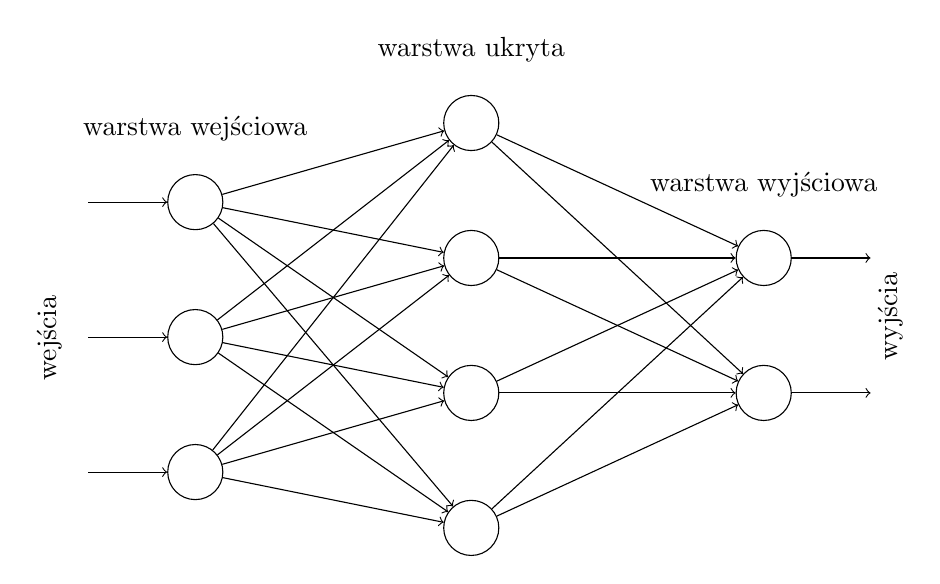
\begin{tikzpicture}[auto,node distance=1.5cm]
	\tikzstyle{node}=[circle,draw]
		\node[node, minimum size=0.7cm, label={[yshift=0.3cm]warstwa wejściowa}] (i1) {$ $};
		\node[node, minimum size=0.7cm] (i2) [below=1.0cm of i1] {$ $};
		\node[node, minimum size=0.7cm] (i3) [below=1.0cm of i2] {$ $};
		\node[node, minimum size=0.7cm, label={[yshift=0.3cm]warstwa ukryta}] (h1) [above right=0.5cm and 3.0cm of i1] {$ $};
		\node[node, minimum size=0.7cm] (h2) [below=1.0cm of h1] {$ $};
		\node[node, minimum size=0.7cm] (h3) [below=1.0cm of h2] {$ $};
		\node[node, minimum size=0.7cm] (h4) [below=1.0cm of h3] {$ $};
		\node[node, minimum size=0.7cm, label={[yshift=0.3cm]warstwa wyjściowa}] (o1) [right= 3.0cm of h2] {$ $};
		\node[node, minimum size=0.7cm] (o2) [below=1.0cm of o1] {$ $};
			\draw[->] (i1) edge node {$ $} (h1);
			\draw[->] (i1) edge node {$ $} (h2);
			\draw[->] (i1) edge node {$ $} (h3);
			\draw[->] (i1) edge node {$ $} (h4);
			\draw[->] (i2) edge node {$ $} (h1);
			\draw[->] (i2) edge node {$ $} (h2);
			\draw[->] (i2) edge node {$ $} (h3);
			\draw[->] (i2) edge node {$ $} (h4);
			\draw[->] (i3) edge node {$ $} (h1);
			\draw[->] (i3) edge node {$ $} (h2);
			\draw[->] (i3) edge node {$ $} (h3);
			\draw[->] (i3) edge node {$ $} (h4);
			\draw[->] (h1) edge node {$ $} (o1);
			\draw[->] (h1) edge node {$ $} (o2);
			\draw[->] (h2) edge node {$ $} (o1);
			\draw[->] (h2) edge node {$ $} (o2);
			\draw[->] (h3) edge node {$ $} (o1);
			\draw[->] (h3) edge node {$ $} (o2);
			\draw[->] (h4) edge node {$ $} (o1);
			\draw[->] (h4) edge node {$ $} (o2);
			\node (input1) [left=1.0cm of i1] {$ $};
			\node[label={[xshift=-0.25cm, yshift=0.65cm, rotate=90]left:wejścia}] (input2) [left=1.0cm of i2] {$ $};
			\node (input3) [left=1.0cm of i3] {$ $};
			\draw[->] (input1) edge node {$ $} (i1);
			\draw[->] (input2) edge node {$ $} (i2);
			\draw[->] (input3) edge node {$ $} (i3);
			\node (output1) [right=1.0cm of o1] {$ $};
			\node[label={[xshift=0.25cm, yshift=1.65cm, rotate=90]left:wyjścia}] (output2) [right=1.0cm of o2] {$ $};
			\draw[->] (o1) edge node {$ $} (output1);
			\draw[->] (o2) edge node {$ $} (output2);
\end{tikzpicture}
	\caption{Schemat sieci neuronowej}
	\label{feedforward-NN}
\end{figure}

Sieci neuronowe to szeroka klasa modeli wykorzystywana najczęściej do zadania uczenia nadzorowanego. W podstawowej formie sieć składa się z wielu warstw neuronów połączonych ze sobą (Rysunek \ref{feedforward-NN}). Warstwa wejściowa sieci odpowiada za przyjmowanie wektorów wejściowych. Neurony w warstwie ukrytej realizują funkcję nieliniową opisaną równaniem:

\begin{equation}
	x_i = f(w_i u_i)
\end{equation}

Gdzie $x_i$ jest wyjściem $i$-tego neuronu w warstwie (nazywanym również aktywacją neuronu), $f$ jest funkcją aktywacji w warstwie do której należy neuron, $w_i$ jest wektorem wag $i$-tego neuronu a $u_i$ jest wektorem wejść $i$-tego neuronu. Nieliniowość całej operacji jest powodowana przez nieliniową funkcję aktywacji. W procesie uczenia definiowana jest funkcja strat (ang. loss function) $L$ opisująca w sposób ilościowy jak bardzo wyjście sieci neuronowej różni się od oczekiwanej wartości. Wartości funkcji strat są wykorzystywane do modyfikacji wag sieci neuronowej (algorytm wstecznej propagacji błędu), najczęściej z wykorzystaniem reguł gradientowych. Dzięki algorytmowi wstecznej propagacji możliwe jest uczenie wielowarstwowych sieci. Wyjście każdej warstwy stanowi zmodyfikowaną reprezentację oryginalnej przestrzeni. Przez nieliniowości i tworzenie reprezentacji przestrzeni cech, wielowarstwowe sieci neuronowe posiadają zdolność do generowania bardzo złożonych granic decyzyjnych.

Sieci neuronowe są stosunkowo starą klasą modeli. Pierwsze prace w zakresie reguł uczenia pojawiły się latach 40. XX wieku \cite{McCulloch-Pitts} \cite{Hebb}. Rosenblat \cite{Rosenblatt} w 1958 roku skonstruował perceptron - maszynę wykazującą zdolność nauki. Uważa się, że publikacja w które zbadano ogarniczenia perpceptoronu i udowodniono, że podejedyncza wartswa sieci nie jest w stanie nauczyć się funkcji XOR \cite{Perceptrons} zaczpoątkowała okres nazwany zimą sztucznej inteligencji (ang. AI Winter). Prawdziwym przełomem okazała się praca \cite{Rumelhart}, w której zaproponowano algorytm wstecznej propagacji błędów. Po publikacji tej zainteresowanie głębokimi sieciami neuronowymi zaczęło wzrastać. W \cite{Conv} zaproponowano warstwy konwolucyjne, które pozwoliły na łatwiejsze przetwarzanie obrazów przez sieci neuronowe. 
Gwałtowny wzrost popularności sieci neuronowych w ostatnich latach można przypisać kilku czynnikom \cite{Goodfellow-et-al-2016}. Pierwszym z nich jest zwiększenie mocy obliczeniowej dostępnej dla praktyków i badaczy uczenia maszynowego, co pozwoliło na zwiększenie rozmiarów modeli i skrócenie czasu uczenia. Drugim czynnikiem jest pojawienie wielu obszernych zbiorów danych, związane z rozpowszechnieniem się internetu i urządzeń elektronicznych w życiu codziennym ludzi. Oba te czynniki pozwalają na skuteczniejsze trenowanie modeli o większych pojemnościach, przeznaczonych do coraz bardziej złożonych zadań. Szczegółowy przegląd historii sieci neuronowych został podany w \cite{DBLP:journals/corr/Schmidhuber14}.

Można dopatrywać się powiązań między sposobem działania ludzkiego mózgu a sieciami neuronowymi. Podobieństwo to może być widoczne w sposobie działania synaps komórki nerowowej. Badacze podkreślają \cite{Goodfellow-et-al-2016}, że związek sieci neuronowych z biologią ma bardziej charakter luźnej inspiracji niż rzeczywistego modelowania zjawisk zachodzących w ludzkim mózgu.

\subsection{Rekurencyjne sieci neuronowe}

\begin{figure}
\centering
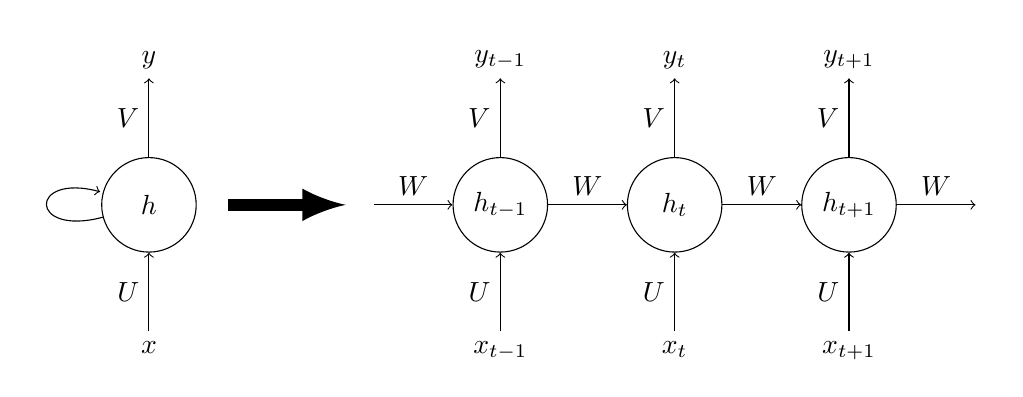
\begin{tikzpicture}[auto,node distance=1.5cm]
	\tikzstyle{node}=[circle,draw]
		\node[node, minimum size=1.2cm] (h) {$h$};
		\draw[->] (h) edge  [loop left] node {$ $} (h);
		\node (o) [above=1.0cm of h] {$y$};
		\node (x) [below=1.0cm of h] {$x$};
			\draw[->] (h) edge node {$V$} (o);
			\draw[->] (x) edge node {$U$} (h);
		\node[right=2.0cm of h] (h0) {$ $};
		\node[node, right=1.0cm of h0, minimum size=1.2cm] (ht_1) {$h_{t-1}$};
		\node (ot_1) [above=1.0cm of ht_1] {$y_{t-1}$};
		\node (xt_1) [below=1.0cm of ht_1] {$x_{t-1}$};
			\draw[->] (h0) edge node {$W$} (ht_1);
			\draw[->] (ht_1) edge node {$V$} (ot_1);
			\draw[->] (xt_1) edge node {$U$} (ht_1);
		\node[node, right=1.0cm of ht_1, minimum size=1.2cm] (ht) {$h_{t}$};
		\node (ot) [above=1.0cm of ht] {$y_{t}$};
		\node (xt) [below=1.0cm of ht] {$x_{t}$};
			\draw[->] (ht_1) edge node {$W$} (ht);
			\draw[->] (ht) edge node {$V$} (ot);
			\draw[->] (xt) edge node {$U$} (ht);
		\node[node, right=1.0cm of ht, minimum size=1.2cm] (ht1) {$h_{t+1}$};
		\node (ot1) [above=1.0cm of ht1] {$y_{t+1}$};
		\node (xt1) [below=1.0cm of ht1] {$x_{t+1}$};
			\draw[->] (ht) edge node {$W$} (ht1);
			\draw[->] (ht1) edge node {$V$} (ot1);
			\draw[->] (xt1) edge node {$U$} (ht1);
		\node (hend) [right=1.0cm of ht1] {$ $};
			\draw[->] (ht1) edge node {$W$} (hend);
			\pgfsetarrowsend{latex} 
			\pgfsetlinewidth{1ex} 
			\pgfpathmoveto{\pgfpoint{1.0cm}{0.0cm}} 
			\pgfpathlineto{\pgfpoint{2.5cm}{0.0cm}} 
			\pgfusepath{stroke} 
			\useasboundingbox (-0.25,-0.25) rectangle (3.75,2.25);
\end{tikzpicture}
\caption{Schemat sieci rekurencyjnej.} (Lewo) sieci rekurencyjne można przedstawić jako jednostkę obliczeniową, która do realizacji obliczeń wykorzystuje wartości uzyskane dla poprzednich kroków. Na rysunku jest to widoczne w formie czarnego kwadratu, oznaczającego opóźnienie czasowe o jeden krok przy neuronie obok normalnych wejść i wyjść. (Prawo) rozwinięta wersja tego samego schematu, przedstawiająca w jaki sposób obliczenia są wykonywane w poszczególnych krokach. Reprezentacja ta pozwala na łatwiejszą analizę zachowań sieci i stosowanych algorytmów. 
	\label{fig:rnn}
\end{figure}


Sieci feedforward posiadają stałą liczbę wejść i wyjść, przez co nie radzą sobie dobrze z przetwarzaniem danych występujących w ciągach (takich jak tekst, dźwięki czy ciągi czasowe). Istnieją podejścia umożliwiające przetwarzanie ciągów przez sieci feedforward, ale nie cechują się wysoką skutecznością. W celu zaadresowania tego problemu powstały sieci rekurencyjne (ang. Recurrent Neural Networks - RNN).
Sieci Rekurencyjne zostały oparte na pracy Rumelharta \cite{RNN}. RNN posiadają ukryty stan, będący wektorem przekazywanym między poszczególnymi krokami czasowymi. Stan jest obliczany przez warstwą ukrytą sieci na podstawie aktualnego wejścia i stanu sieci z poprzedniego kroku czasowego - Rysunek \ref{fig:rnn}.
Algorytm uczenia RNN - propagacja wsteczna w czasie (ang. Back-Propagation Through Time - BPTT) został przedstawiony w \cite{BPTT}.
Udowodniono, że przy spełnieniu pewnych założeń RNN są kompletne w sensie Turinga \cite{turing-complete}.

\subsubsection{Sieci dwukierunkowe}

Wprowadzono wiele modyfikacji w zakresie zasad działania i struktury RNN. 
W \cite{bidirectional} wprowadzono sieci dwukierunkowe przetwarzające sekwencje w dwóch kierunkach: od początku do końca i od końca do początku. Ostateczna wartość aktywacji dla n-tego elementu sekwencji jest obliczana na podstawie n-tych aktywacji dla obu kierunków.

\subsubsection{LSTM}

RNN w swojej natywnej formie nie są w stanie nauczyć się długich zależności w ciągu uczącym. Problem ten jest w znacznej mierze spowodowany wybuchającymi lub znikającymi gradientami (exploding or vanishing gradients) \cite{vanishing_gradient_RNN}. W celu zaadresowania tego problemu Hochreiter i Schmidhuber zaproponowali architekturę Long Short-Term Memory (LSTM) \cite{LSTM}. Ze względu na swoją strukturę LSTM jest w stanie operować na danych z długimi zależnościami czasowymi. LSTM została dokładniej opisana w dalszej części pracy. 

\subsubsection{GRU}

Gated Recurrent Unit (GRU) \cite{DBLP:journals/corr/ChoMGBSB14} jest modyfikacją LSTM. W wyniku zastosowanych uproszeńw strukturze komórki GRU wymaga mniejszej mocy obliczeniowej do treningu, kosztem mniej mocy modelu. LSTM i GRU uzyskują porównywalne wyniki w praktycznych zastosowaniach \cite{DBLP:journals/corr/ChungGCB14}. GRU została dokładniej opisana w dalszej części pracy.

\subsection{Zadanie klasyfikacji}

Uczenie nadzorowane (ang. supervised learning) to dział uczenia maszyn w którym zbiór uczący składa się z par $\{x, d\}_{i=1}^N$, gdzie $x$ to wektor cech, $d$ to etykieta, a $N$ to liczność zbioru uczącego. W przypadku gdy każdej cechy istnieje osobna etykieta mówimy o silnym etykietowaniu. Gdy jedna etykieta opisuje wszystkie cechy z przykładu uczącego mówimy o słabym etykietowaniu. Przykładowo jeśli zadanie polega na rozpoznaniu samochodu na zdjęciu, mówimy o słabym etykietowaniu. Jeśli zadanie polega na zaznaczeniu wszystkich pikseli przedstawiających samochód na zdjęciu, mówimy o silnym etykietowaniu. Aby określić jakość działania algorytmu wprowadza się funkcję straty dla całego zbioru:

\begin{equation}
	\mathcal{L} = \sum_{i=1}^N L_i
\end{equation}

gdzie $L_i$ to wartość funkcji strat dla pojedynczego przykładu uczącego. Zadanie klasyfikacji opiera się na przypisaniu przykładu uczącego $x$ do odpowiedniej klasy $k$. W procesie uczenia wybieramy hipotezę z przestrzeni hipotez $h \in \mathcal{H}$, która minimalizuje liczbę błędnie zaklasyfikowanych przykładów \cite{introduction-to-machine-learning}. Można to zapisać za pomocą 0-1 funkcji strat:

\begin{equation}
	E(x, d) = \sum_{i=1}^N 1(h(x_i) \neq d_i )
\end{equation}

gdzie $1(x)$ jest równe 1, gdy x jest prawdziwe i 0 gdy x nie jest prawdziwe. 0-1 funkcja strat może być stosowana, gdy na wyjściu klasyfikatora znajduje się etykieta klasy. W przypadku gdy na wyjściu modelu znajduje się prawdopodobieństwo przynależności do klasy często stosowaną funkcją strat jest entropia krzyżowa (ang. cross entropy):

\begin{equation}
	H(h,d) = - \sum h(x) log(d)
\end{equation}

Reguła decyzyjna w takim przypadku opiera się na wyborze najbardziej prawdopodobnej klasy:

\begin{equation}
	h(x) = arg \; \stackunder{max}{k} \; p(C_k | x)
\end{equation}

gdzie $x_i$ to $i$-ty element wektora, będącego argumentem funkcji softmax.

W przypadku sieci neuronowych często stosowaną mechaniką jest wykorzystywanie funkcji softmax w warstwie wyjściowej sieci. Funkcja softmax pozwala na konwertowanie wyjść sieci na prawdopodobieństwa i jest dana wzorem:

\begin{equation}
	softmax(x)_i = \frac{e^{x_i}}{\sum_{k=1}^{K} e^{x_k}}
\end{equation}

Algorytmy klasyfikacji dostosowane dla sieci rekurencyjnych takie jak Connectionist Temporal
Classification zostały szczegółowo omówione w \cite{graves-phd}. W przypadku tej pracy ich wymaganie nie będzie wskazane, ze względu na charakter wykorzystanej architektury sieci.

\section{Przegląd literatury}

W tej sekcji dokonano przeglądu typowych zastosowań sieci rekurencyjnych oraz omówiono prace, w których dokonywano klasyfikacji obrazów za pomocą RNN.

\subsection{Zastosowania rekurencyjnych sieci neuronowych}

Sieci Rekurencyjne znalazły wiele zastosowań w przetwarzaniu sekwencji. 
Jednym z nich może być przetwarzanie języka naturalnego (natural language processing - NLP), gdzie RNN znalazły zastosowanie w rozpoznawaniu mowy \cite{DBLP:journals/corr/abs-1303-5778}, \cite{speech_recognition}, \cite{speech_recognition1}, tłumaczeniu \cite{translate}, \cite{DBLP:journals/corr/ChoMGBSB14}, \cite{DBLP:journals/corr/BahdanauCB14}, \cite{DBLP:journals/corr/WuSCLNMKCGMKSJL16}, modelowniu języka \cite{DBLP:journals/corr/ChoMGBSB14}, generowaniu mowy \cite{DBLP:journals/corr/MehriKGKJSCB16} i generowaniu tekstu \cite{DBLP:journals/corr/Graves13} \cite{karpathy_RNN_blog}. 
Innym polem zastosowań RNN jest rozpoznawanie pisma ręcznego \cite{handwriting_recognition}, \cite{handwriting_recognition2} lub jego generacja \cite{DBLP:journals/corr/Graves13}.
RNN są także wykorzystywane do generowania obrazów \cite{DBLP:journals/corr/GregorDGW15} i muzyki \cite{DBLP:journals/corr/abs-1804-07300}.
Autorzy \cite{DBLP:journals/corr/VinyalsL15} zaproponowali system do przeprowadzania rozmów zbudowany z wykorzystaniem RNN.

Sieci rekurencyjne są także wykorzystywane w połączeniu z innymi modelami np. w połączeniu z CNN w celu generowania podpisów dla obrazów \cite{DBLP:journals/corr/VinyalsTBE14}, gdzie CNN jest wykorzystywane do klasyfikacji obrazu i przygotowywania reprezentacji obrazu w architekturze encoder-decoder, a RNN generuje podpis obrazka.

\subsection{Zastosowanie sieci rekurencyjnych do klasyfikacji obrazów}

W \cite{DBLP:journals/corr/VisinKCMCB15} wykorzystano sieć rekurencyjną do klasyfikacji obrazów. Proponowany model ReNet wykorzystuje RNN do czterotnego trawersowania fragmentów obrazu w celu ekstrakcji cech, jako alternatywę dla warstw konwolucyjnych z poolingiem. W \cite{DBLP:journals/corr/abs-0705-2011} wprowadzono wielowymiarowe sieci rekurencyjne, które obliczały aktywację w danej komórce nie tylko na podstawie aktywacji z poprzedniej iteracji, ale także na podstawie wartości aktywacji sąsiadujących komórek w aktualnym kroku czasowym. Model wielowymiarowych RNN został wykorzystany w przypadku tej pracy do przeprowadzenia segmentacji obrazu. Idea ta została rozwinięta w \cite{DBLP:journals/corr/KalchbrennerDG15}, gdzie przedstawiono Grid LSTM. Jest to model rozszerzający standardowy model sieci LSTM do N-wymiarowych komórek ze współdzielonymi wektorami stanu i pamięci. Wielowymiarowe sieci rekurencyjne stanowią ciekawą klasę modeli, mogą jednak wymagać znaczących zasobów mocy obliczeniowej do przeprowadzenia procesu uczenia.

\section{Cel pracy}

Celem pracy jest zbadanie skuteczności klasyfikacji zmodyfikowanej architektury ReNet. Proponowana modyfikacja polega na zastąpieniu czterech sieci rekurencyjnych dwiema sieciami rekurencyjnymi analizącymi obraz skonwertowany do jednowymiarowego ciągu otrzymanego z wykorzystaniem krzywych wypełniającej przestrzeń (ang. space-filling curves). Wyniki klasyfikacji wybranego zbioru danych zostaną porównane z oryginalną architekturą oraz wynikami osiąganymi dla sieci konwolucyjnych. Wykorzystanie dwóch sieci rekurencyjnych zamiast czterech powinno pozwolić na zmniejszenie liczby parametrów modelu. Mniejsza liczba parametrów może przekładać się na krótszy czas szkolenia i może pozwolić wykorzystanie modelu z większą liczbę neuronów w warstwach ukrytych modelu. Modyfikacja sieci będzie mieć wpływ na zdolność uczenia sieci, co oczywiście jest najciekawszym przedmiotem badań. 


W zakres eksperymentów będzie wchodziło również zbadanie wpływu różnych architektur sieci rekurencyjnych na uzyskiwane wyniki. Hiperparametry modeli zostaną dobrane z wykorzystaniem podziału zbioru danych na zbiór uczący i zbiór testowy. Do doboru wartości hiperparametrów zostanie wykorzystany algorytm wyszukiwania sieciowego (ang. grid search) z modyfikacją polegającą na zastąpieniu przeszukiwania zupełnego przez przeszukiwanie zachłanne. Dokładność klasyfikacji zostanie zmierzona z wykorzystaniem dokładności na zbiorze testowym (ang. accuracy) i algorytmowi sprawdzianu krzyżowego. Po wprowadzeniu najistotniejszych terminów wykorzystywanych w dalszych częściach pracy oraz nakreśleniu problematyki w następnym rozdziale zostaną dokładniej omówione teoretyczne aspekty wprowadzonych pojęć.


\chapter{Omówienie wybranych zagadnień teoretycznych}

W rozdziale tym zostały omówione teoretyczne podstawy wybranych algorytmów i struktur sieci, wykorzystanych w badaniach.

\section{Rekurencyjna Sieć Neuronowa}

Sieci rekurencyjne są modyfikacją zwykłych sieci feedforward powstałą poprzez dopuszczenie możliwości powstawania cykli w grafie obliczeniowym. Aktywacja każdej jednostki może być wyrażona jako:


\begin{equation}
	h_t = F(h_{t-1}, x_t)
	\label{eq:basic-rnn}
\end{equation}

gdzie $h_t$ to aktywacja jednostki w czasie $t$, $x_t$ to wejście jednostki w czasie $t$, a $F$ oznacza przekształcenie realizowane przez jednostkę obliczeniową. Takie sformułowanie zasady działania modelu jest realizacją współdzielenia parametrów przez części modelu. Każda jednostka do obliczenia aktywacji wykorzystuje aktualne wejście i aktywację z poprzedniego kroku. Aby uniezależnić model od długości sekwencji wykorzystuje się ten sam zestaw parametrów w każdym kroku.

Aktywacja może zostać wykorzystana do obliczenia wartości wyjścia $y_t$:

\begin{equation}
	y_t = G(h_t)
\end{equation}

gdzie $G$ oznacza nieliniowe przekształcenie realizowane przez warstwę wyjściową sieci.

W trakcie uczenia sieci dokonuje się rozwinięcia (ang. unfolding) grafu obliczeniowego, poprzez wielokrotne zastosowanie definicji sieci. Przykładowo dla dwóch kroków w czasie odwinięcie grafu można zapisać jako:

\begin{equation}
	h_2 = F(h_1, x_2) = F(F(h_0, x_1), x_2)
\end{equation}

\begin{figure}[h]
\centering
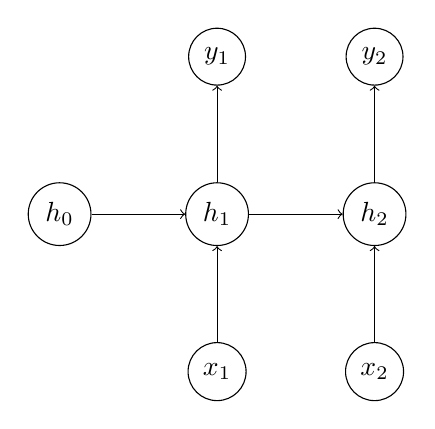
\begin{tikzpicture}[auto,node distance=2.0cm]
	\tikzstyle{node}=[circle,draw]
		\node[node] (h0) {$h_0$};
		\node[node] (h1) [right of=h0] {$h_1$};
		\node[node] (x1) [below of=h1] {$x_1$};
		\node[node] (y1) [above of=h1] {$y_1$};
		\node[node] (h2) [right of=h1] {$h_2$};
		\node[node] (x2) [below of=h2] {$x_2$};
		\node[node] (y2) [above of=h2] {$y_2$};
			\draw[->] (h0) edge node {$ $} (h1);
			\draw[->] (x1) edge node {$ $} (h1);
			\draw[->] (h1) edge node {$ $} (y1);
			\draw[->] (h1) edge node {$ $} (h2);
			\draw[->] (x2) edge node {$ $} (h2);
			\draw[->] (h2) edge node {$ $} (y2);
\end{tikzpicture}
\caption{Schemat rozwiniętego grafu obliczeniowego sieci rekurencyjnej.}
\label{fig:unfolded}
\end{figure}

Co jest dwukrotnym zastosowaniem równania \ref{eq:basic-rnn} rekurencyjnie. Jako początkowy stan sieci $h_0$ najczęściej stosowany jest wektor zer. Rozwinięcie grafu pozwala na zamianę grafu cyklicznego na acykliczny, bardziej przypominający graf sieci feedforward. Przykładowy rozwinięty graf przedstawiono na rysunku \ref{fig:unfolded}. Rozwinięty graf pozwala na zastosowanie reguł propagacji wstecznej i obliczenie gradientów funkcji strat. Jest więc to proces umożliwiający uczenie sieci rekurencyjnej.

\begin{figure}
\centering
	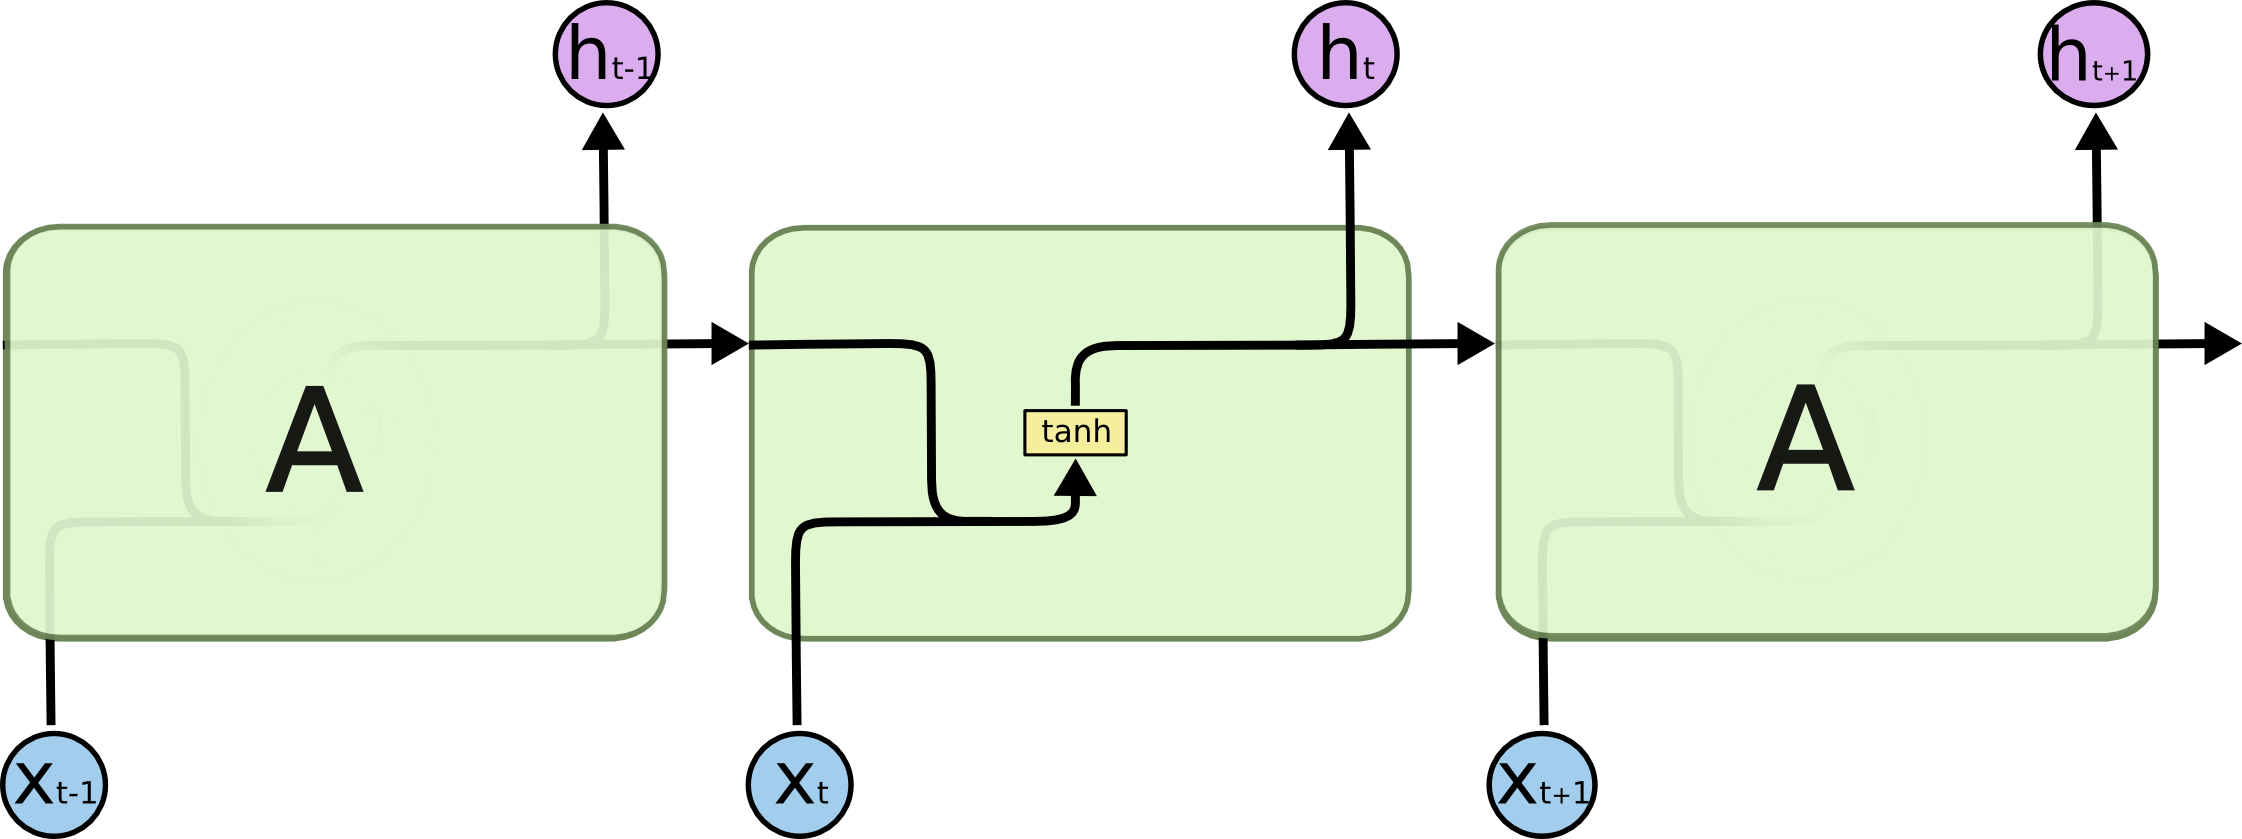
\includegraphics[width=0.9\textwidth]{img/LSTM3-SimpleRNN.png}
	\caption{Schemat podstawowej jednostki sieci rekurencyjnej, korzystającej z funkcji aktywacji $tanhh$.} Źródło: \cite{colah}.
	\label{fig:simple_rnn}
\end{figure}

Przekształcenie realizowane przez pojedynczą ukrytą jednostkę RNN w najbardziej podstawowej formie można zapisać jako:

\begin{equation}
	h_t = f(W h_{t-1} + U x_t + b_u)
\end{equation}

gdzie $W$ i $U$ to macierze wag, $b_u$ to wektor biasu, a $f$ to funkcja aktywacji. Najczęściej stosowanymi funkcjami aktywacji są funkcja sigmoidalna, tanh lub ReLU.

Przekształcenie realizowane przez pojedynczą jednostkę wyjściową można zapisać jako:

\begin{equation}
	y_t = g(Y h_t + b_y)
\end{equation}

gdzie $Y$ to macierz wag, $b_y$ to wektor biasu, a $g$ to funkcja aktywacji. Najczęściej stosowaną funkcją w warstwie wyjściowej jest softmax.

Istnieje wiele modyfikacji wprowadzonych do struktury jednostki sieci rekurencyjnej, które zostały omówione w dalszej części rozdziału.

\section{Propagacja wsteczna w czasie}

Propagacja wsteczna w czasie to algorytm dedykowany do uczenia sieci rekurencyjnych. Polega on na wykorzystaniu rozwiniętej formy grafu obliczeniowego sieci rekurencyjnej i zastosowaniu propagacji wstecznej, z uwzględnieniem faktu współdzielenia parametrów - każda jednostka rekurencyjna korzysta z tego samego zestawu parametrów.

\begin{figure}
\centering
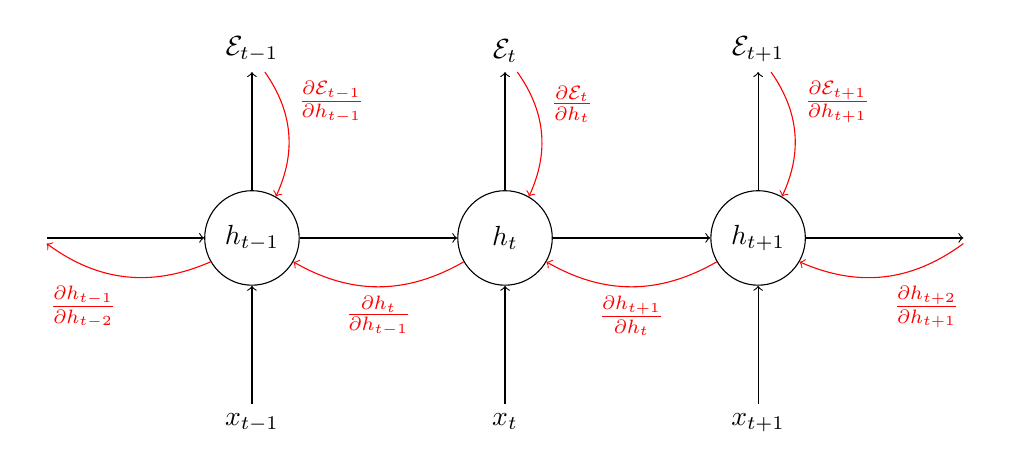
\begin{tikzpicture}[auto,node distance=1.5cm]
	\tikzstyle{node}=[circle,draw]
		\node (h) {$ $};
		\node[node, right=2.0cm of h, minimum size=1.2cm] (ht_1) {$h_{t-1}$};
		\node (ot_1) [above=1.5cm of ht_1] {$\mathcal{E}_{t-1}$};
		\node (xt_1) [below=1.5cm of ht_1] {$x_{t-1}$};
			\draw[->] (h) edge node {$ $} (ht_1);
			\draw[->] (ht_1) edge node {$ $} (ot_1);
			\draw[->] (xt_1) edge node {$ $} (ht_1);
			\draw[->, bend left=30, red] (ot_1) edge node {$\frac{\partial \mathcal{E}_{t-1}}{\partial h_{t-1}}$} (ht_1);
			\draw[->, bend left=30, red] (ht_1) edge node {$\frac{\partial h_{t-1}}{\partial h_{t-2}}$} (h);
		\node[node, right=2.0cm of ht_1, minimum size=1.2cm] (ht) {$h_{t}$};
		\node (ot) [above=1.5cm of ht] {$\mathcal{E}_{t}$};
		\node (xt) [below=1.5cm of ht] {$x_{t}$};
			\draw[->] (ht_1) edge node {$ $} (ht);
			\draw[->] (ht) edge node {$ $} (ot);
			\draw[->] (xt) edge node {$ $} (ht);
			\draw[->, bend left=30, red] (ot) edge node {$\frac{\partial \mathcal{E}_{t}}{\partial h_{t}}$} (ht);
			\draw[->, bend left=30, red] (ht) edge node {$\frac{\partial h_{t}}{\partial h_{t-1}}$} (ht_1);
		\node[node, right=2.0cm of ht, minimum size=1.2cm] (ht1) {$h_{t+1}$};
		\node (ot1) [above=1.5cm of ht1] {$\mathcal{E}_{t+1}$};
		\node (xt1) [below=1.5cm of ht1] {$x_{t+1}$};
			\draw[->] (ht) edge node {$ $} (ht1);
			\draw[->] (ht1) edge node {$ $} (ot1);
			\draw[->] (xt1) edge node {$ $} (ht1);
			\draw[->, bend left=30, red] (ot1) edge node {$\frac{\partial \mathcal{E}_{t+1}}{\partial h_{t+1}}$} (ht1);
			\draw[->, bend left=30, red] (ht1) edge node {$\frac{\partial h_{t+1}}{\partial h_{t}}$} (ht);
		\node (h_end) [right=2.0cm of ht1] {$ $};
			\draw[->] (ht1) edge node {$ $} (h_end);
			\draw[->, bend left=30, red] (h_end) edge node {$\frac{\partial h_{t+2}}{\partial h_{t+1}}$} (ht1);
\end{tikzpicture}
\caption{Schemat działania propagacji wstecznej w czasie.} Czarnym kolorem zaznaczono przepływ informacji przy obliczaniu aktywacji sieci (forward pass). Czerwonym kolorem zaznaczono przepływ informacji przy zastosowaniu wstecznej propagacji błędu.
	\label{fig:rnn_backprop}
\end{figure}

Błąd propagowany wstecz dla każdego kroku $\mathcal{E}_t$ można zapisać jako wartość funkcji strat $\mathcal{L}$ od aktywacji w danym kroku $h_t$:

\begin{equation}
	\mathcal{E}_t = \mathcal{L}(h_t)
\end{equation}

Ze względu na współdzielenie parametrów sieci rekurencyjnej w każdym kroku czasowym gradient względem wybranego parametru sieci $\theta$ jest sumą gradientów dla każdego kroku w ciągu uczącym osobno:

\begin{equation}
	\frac{\partial \mathcal{E}}{\partial \theta} = \sum_{1 \leq t \leq T} \frac{\partial \mathcal{E}_t}{\partial \theta}
\end{equation}

gdzie $T$ to długość sekwencji w ciągu uczącym. Wartość gradientu dla każdego kroku czasowego wyznacza się stosując regułę łańcucha dla pochodnych przy cofaniu się wzdłuż grafu obliczeniowego, tak jak ma to miejsce dla propagacji wstecznej:

\begin{equation}
	\frac{\partial \mathcal{E}_t}{\partial \theta} = \sum_{1 \leq k \leq t} (\frac{\partial \mathcal{E}_t}{\partial h_t} \frac{\partial h_t}{\partial h_k} \frac{\partial h_k}{\partial \theta})
\end{equation}

Suma w powyższym wzorze określa wpływ parametrów sieci w czasie $k$ poprzedzającym $t$ lub w samej chwili $t$ na aktualną wartość wyjścia w czasie $t$. Wyrażenie $\frac{\partial \mathcal{E}_t}{\partial h_t}$ można zapisać stosując regułę łańcucha jako:

\begin{equation}
	\frac{\partial \mathcal{E}_t}{\partial h_t} = \frac{\partial \mathcal{E}_t}{\partial y_t} \frac{\partial y_t}{\partial h_t} = \frac{\partial \mathcal{E}_t}{\partial h_t} \frac{\partial g(outnet_t)}{\partial outnet_t} Y
\end{equation}

gdzie $outnet_t = Y h_t + b_y$ Wyrażenie $\frac{\partial h_t}{\partial h_k}$ można zapisać ponownie stosując regułę łańcucha jako:

\begin{equation}
	\frac{\partial h_t}{\partial h_k} = \prod_{k < i \leq t} \frac{\partial h_i}{\partial h_{i-1}} = \prod_{k < i \leq t} diag( \frac{\partial f(net_i)}{\partial net_i}) W
\label{eq:BPTT_product}
\end{equation}

gdzie $net_i = W h_i + U x_i + b_u$. Działanie wstecznej propagacji w czasie zostało zilustrowane na rysunku \ref{fig:rnn_backprop}. Powyższe rozważania zostały przeprowadzone dla najprostszej jednostki RNN, ale ilustruję ideę działania. Dla bardziej skomplikowanych jednostek idea ta pozostaje niezmienna. Nadal wykorzystywana jest rozwinięta forma grafu obliczeniowego do obliczenia błędu, połączona z faktem współdzielenia parametrów. 

Problemy związane z propagacją wsteczną w czasie zostały omówione w \cite{DBLP:journals/corr/abs-1211-5063}. Najbardziej istotny problem jest związany z iloczynem w równaniu \ref{eq:BPTT_product}. Wielokrotne mnożenie gradientów o module $|\frac{\partial h_i}{\partial h_{i-1}}| < 1$ powoduje problem znikających gradientów. Analogicznie wielokrotne mnożenie gradientów o module $|\frac{\partial h_i}{\partial h_{i-1}}| > 1$ powoduje problem wybuchających gradientów. W równaniu \ref{eq:BPTT_product} różnica $t - k$ oznacza czas pomiędzy aktualną jednostką a jednostką, której wpływ właśnie analizujemy. Wraz ze zwiększającym się $t - k$, liczba kolejnych mnożeń wzrasta. Jest to powodem znacznych trudności w uczeniu się długich zależności czasowych przez sieć.  Dyskusja możliwych rozwiązań została podana w \cite{DBLP:journals/corr/abs-1211-5063}. W pracy tej zastosowano inną definicję $h_t$, przez co część rozważań teoretycznych traci na ważności w kontekście definicji $h_t$ zastosowanej w tej pracy. Niemniej jednak część rozważań można zastosować dla parametryzacji przyjętej w tej pracy.

W pierwszej kolejności należy zapisać jakobian z równania \ref{eq:BPTT_product} jako:

\begin{equation}
	\frac{\partial h_t}{\partial h_{t-1}} = diag(g'(W h_{t-1} + Ux_{t} + b)) W
\end{equation}

Przyjmijmy, że $\gamma$ oznacza górne ograniczenie 2-normy macierzy $diag(g'(W h_{t-1} + Ux_{t} + b))$:
\begin{equation}
	||diag(g'(W h_{t-1} + Ux_{t} + b))||_2 \leq \gamma
\end{equation}

Następnie korzystając z nierówności trójkąta można zapisać:

\begin{equation}
	\forall_{t} ||\frac{\partial h_{t}}{\partial h_{t-1}}||_2 \leq ||diag(g'(W h_{t-1} + Ux_{t} + b))||_2 ||W||_2 
\end{equation}

Jeśli największa wartość własna $\lambda_{1}$ macierzy $W$ (wartość 2-normy) spełnia warunek:

\begin{equation}
	|\lambda_{1}| < \frac{1}{\gamma}
\end{equation}

to wtedy zachodzi:

\begin{equation}
	\forall_{t} ||\frac{\partial h_{t}}{\partial h_{t-1}}||_2 \leq \gamma \frac{1}{\gamma} = 1
\end{equation}

co oznacza, że przy obliczaniu iloczynu jakobianów w równaniu \ref{eq:BPTT_product} uzyskamy jako wynik bardzo małe wartości i nastąpi znikanie gradientów. Analogiczne rozumowanie może zostać przeprowadzone dla wybuchających gradientów i zmienionej definicji $\gamma$. W dwóch pozostałych sekcjach tego rozdziału omówiono struktury komórki sieci rekurencyjnej, które pozwalają na uniknięcie problemu znikających gradientów. 


\section{LSTM}

\begin{figure}
\centering
	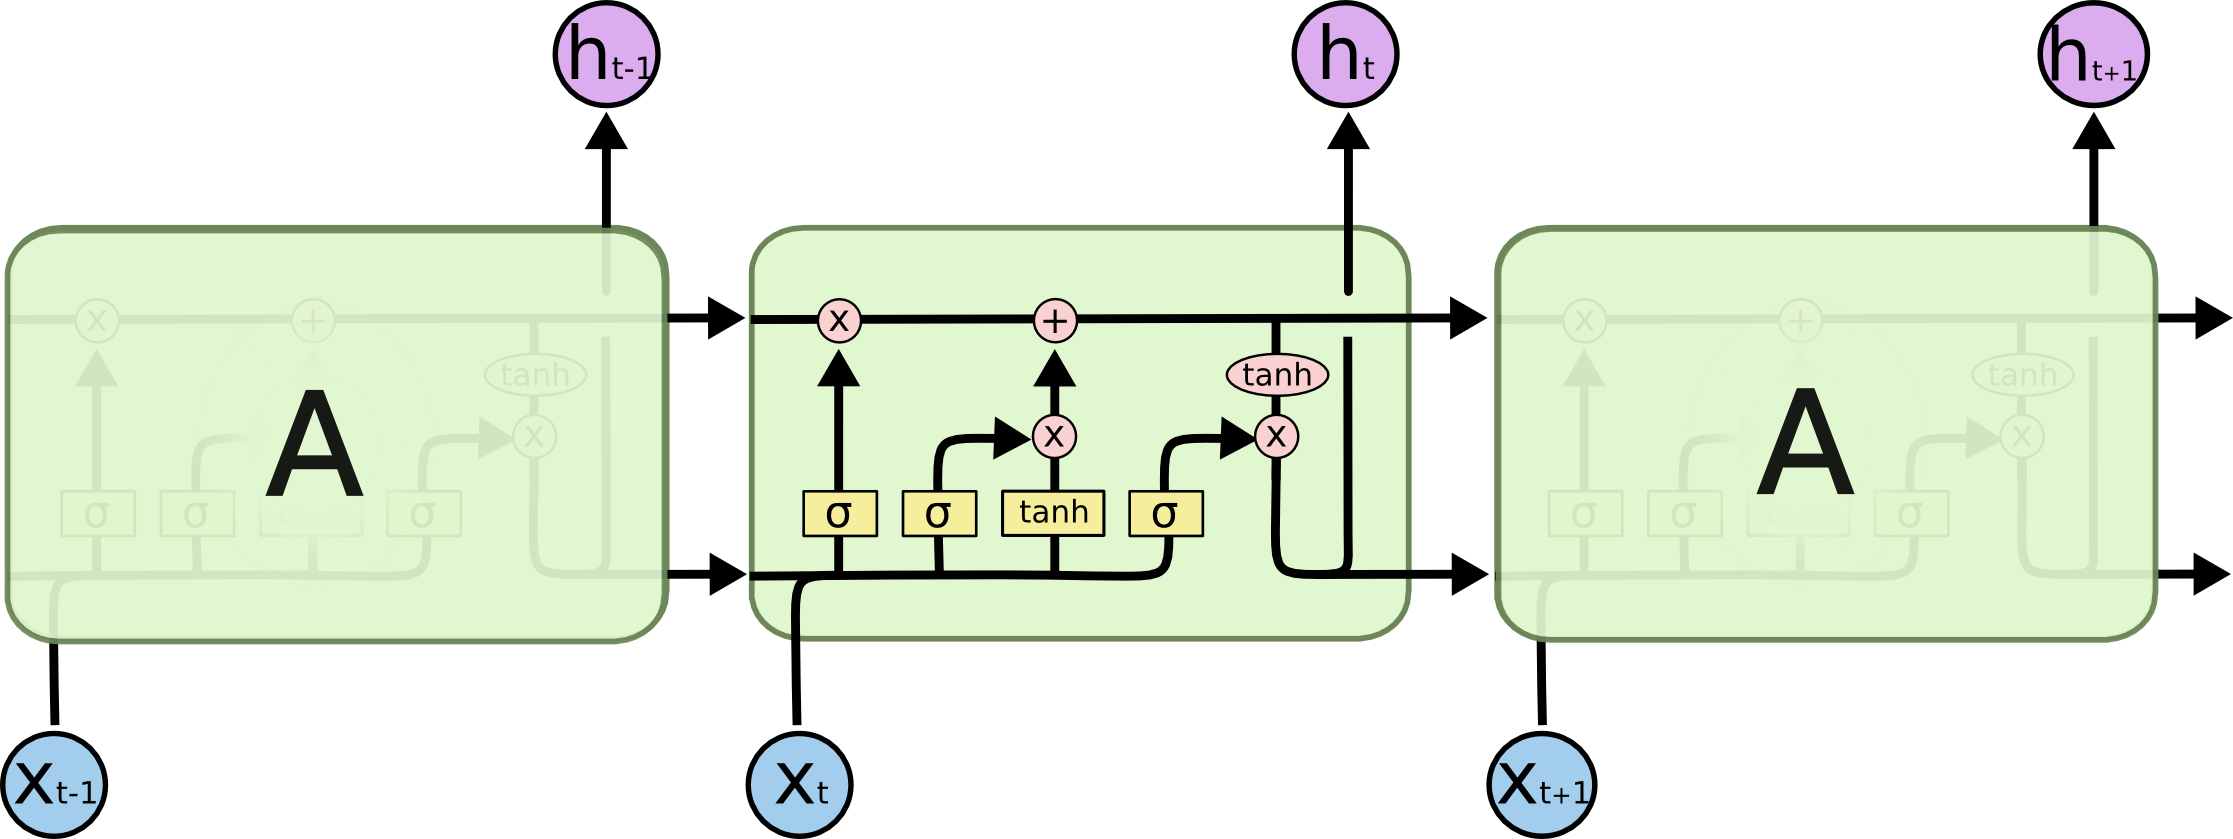
\includegraphics[width=0.90\textwidth]{img/lstm_colah.png}
	\caption{Schemat komórki LSTM.} Źródło: \cite{colah}.
	\label{fig:lstm}
\end{figure}

LSTM jest jedną z popularniejszych architektur RNN. Hochreiter i Schmidhuber zaproponowali architekturę Long Short-Term Memory (LSTM) \cite{LSTM} w 1997. Zwykła sieć RNN składa się jedynie ze stanu sieci $h$, oraz wejścia $x$. Obie te wartości są wejściem warstwy ukrytej sieci. Wyjście warstwy ukrytej jest wyjściem sieci. Struktura komórki LSTM jest bardziej skomplikowana i składa się z wektora stanu sieci $h$, komórki pamięci $C$, oraz czterech ukrytych warstw sieci. Schemat ze strukturą sieci został przedstawiony na rysunku \ref{fig:lstm}.

Warstwy sieci LSTM z sigmoidalnymi funkcjami aktywacji są nazywane bramkami multiplikatywnymi. Sigmoidalna funkcja aktywacji jest opisywana za pomocą wzoru:

\begin{equation}
	\sigma(x) = \frac{1}{e^{-x} + 1}
\end{equation}

i posiada zbiór wartości $(0, 1)$. Przemnożenie wyjścia tej warstwy z dowolną wartością powoduje jej przeskalowanie, przez co warstwy te są wykorzystywane do kontrolowania wartości zmiennych komórki LSTM. Dodatkowo bramki jako warstwy sieci posiadają wagi, które ulegają modyfikacji w trakcie uczenia, przez co LSTM w procesie uczenia zyskują informację o tym kiedy i w jaki sposób uaktualnić swój stan i komórkę pamięci na podstawie obecnie posiadanych informacji. Wyróżnia się 3 bramki. Pierwszą z nich jest forget gate. Jest ona odpowiedzialna za zmniejszanie wartości aktualnie znajdującej się w komórce pamięci. Operacja realizowana przez forget gate jest opisywana wzorem: 

\begin{equation}
	f_t = \sigma( W_f [ h_{t-1}, x_t ] + b_f )
\end{equation}

Gdzie $W_f$ i $b_f$ to odpowiednio wagi i bias warstwy, $h_{t-1}$ to stan komórki z poprzedniego kroku, a $x_t$ to aktualne wejście sieci. Kolejną bramką jest input gate. Realizowana operacja wyraża się analogicznym wzorem:

\begin{equation}
	i_t = \sigma( W_i [ h_{t-1}, x_t ] + b_i )
\end{equation}

Intuicyjnie jest ona odpowiedzialna za określanie w jakim stopniu należy zaktualizować komórkę pamięci sieci na podstawie aktualnego wejścia sieci $x_t$ i stanu z poprzedniego kroku $h_{t-1}$. Na podstawie $x_t$ i $h_{t-1}$ jest obliczana wartość $\tilde{C}_t$:

\begin{equation}
	\tilde{C}_t = tanh( W_c [ h_{t-1}, x_t ] + b_C )
\end{equation}

Wartość $\tilde{C}_t$ może być określona jako kandydat do zastąpienia stanu komórki z poprzedniego kroku $C_{t-1}$. Aktualna wartość $C_t$ jest zatem obliczana ze wzoru:

\begin{equation}
	C_t = f_t \odot C_{t-1} + i_t \odot \tilde{C}_t
\end{equation}

gdzie $\odot$ oznacza iloczyn Hadamarda (iloczyn wszystkich odpowiadających sobie elementów wektora lub macierzy). Ostatnią bramką jest output gate. Realizowana operacja jest dana wzorem:

\begin{equation}
	o_t = \sigma( W_o [ h_{t-1}, x_t ] + b_o )
\end{equation}

Bramka ta służy do określania sposobu w jaki zostanie zaktualizowany stan $h$ w aktualnym kroku $t$, co wyraża się równaniem:

\begin{equation}
	h_t = o_t \odot tanh( C_t )
\end{equation}

\begin{figure}
\centering
	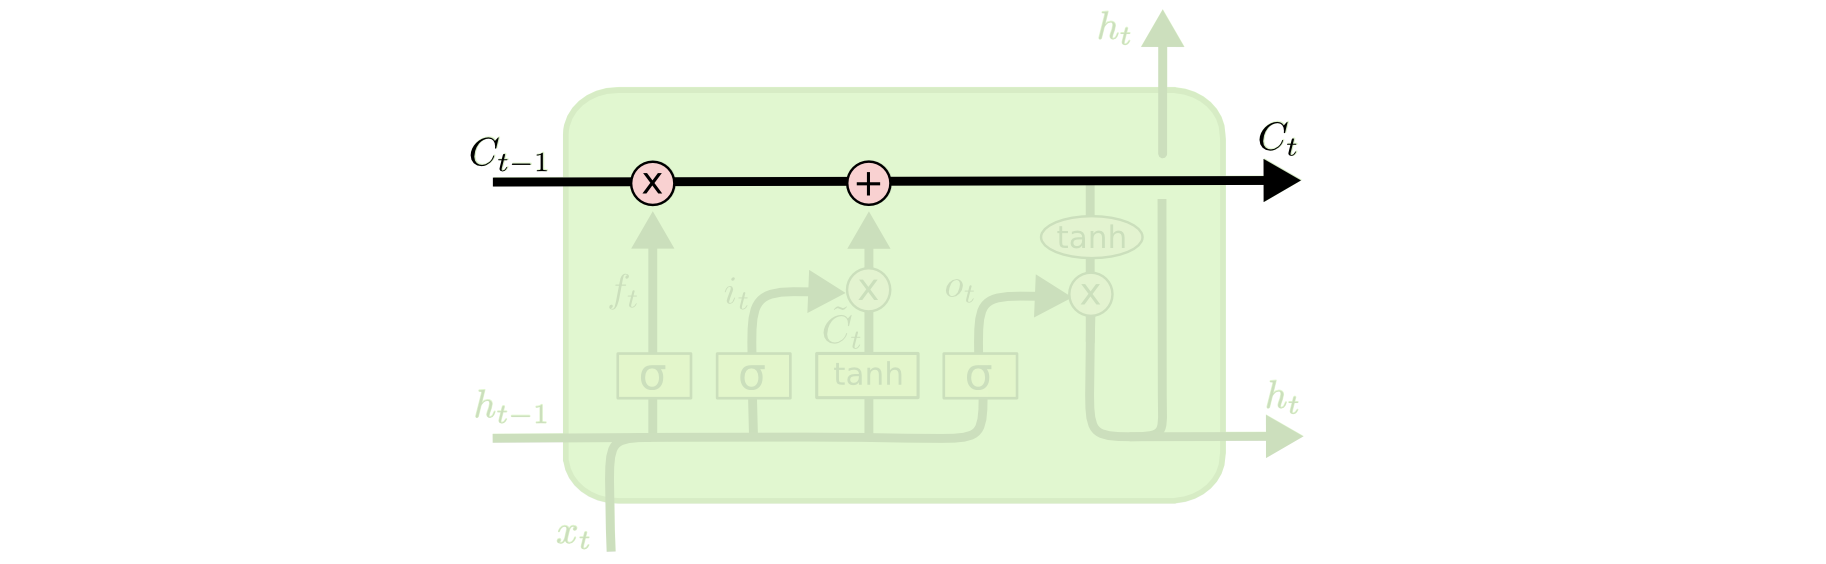
\includegraphics[width=0.90\textwidth]{img/LSTM3-C-line.png}
	\caption{Schemat komórki LSTM z zaznaczoną komórką pamięci.} W przypadku propagacji wstecznej przy cofaniu się przez graf obliczeniowy sieci węzły odpowiadające operacji dodawania propagują wartość błędu bez modyfikacji wartości. Węzły w grafie odpowiadające operacji mnożenia powodują przemnożenie wartości dotychczasowego błędu przez drugi argument. W tym przypadku realizowana operacja to $C_t = f_t \odot C_{t-1} + i_t \odot \tilde{C}_t$. W wyniku propagacji wstecznej uzyskujemy pochodną $\frac{\partial L}{\partial C_t}$. Opearcja dodawnia nie zmienia wartość błędu, więc $\frac{\partial L}{\partial (f_t \odot C_{t-1})} = \frac{\partial L}{\partial C_t}$. Przy operacji mnożenia pochodna cząstkowa względem $C_{t-1}$ wynosi $\frac{\partial C_t}{\partial C_{t-1}} = f_t$. Błąd propagowany przez komórkę pamięci ma ostateczną wartość: $\frac{\partial L}{\partial C_{t-1}} = \frac{\partial L}{\partial C_t} f_t$. Ze względu na zbiór wartości funkcji sigmoidalnej $f_t \in (0, 1)$ wartość propagowanego błędu nadal jest pomniejszana w każdym kroku. Intuicyjnie wartość błędu jest zmniejszana w takim samym stopniu jak wartość sygnału przy normalnym przejściu przez forget gate (decyzja w jakim stopniu informacje nie są istotne w aktualnym kontekście). Zaproponowana architektura unika jednakże obliczania pochodnej względem funkcji aktywacji sigmoidalnej (pochodna funkcji sigmoidalnej: $\frac{d \sigma}{dx} = \sigma (x)(1 - \sigma (x)$) przy propagacji wstecznej błędu, co powoduje wolniejsze zmniejszanie wartości sygnału błędu. Źródło: \cite{colah}. 
	\label{fig:lstm-mem-cell}
\end{figure}

Warto zwrócić uwagę, że w powyższym równaniu nie występują wagi ani bias, więc $tanh$ nie jest utożsamiony z warstwą sieci neuronowej.

W swojej pracy \cite{LSTM} Hochreiter i Schmidhuber odnoszą się do wcześniejszej pracy \cite{vanishing_gradient_RNN}, gdzie zostały przeanalizowane źródła problemów związanych ze znikającymi gradientami. Jako główny problem został wskazany gradient względem dowolnej zmiennej $a$ w grafie obliczeniowym $|\frac{\partial L}{\partial a}| > 1.0$ powodujący wybuchanie wag, lub $|\frac{\partial L}{\partial a}| < 1.0$ powodujący znikanie wag. W strukturze LSTM komórka pamięci jest sposobem zapobiegania temu problemowi. Komórka pamięci przy propagacji wstecznej pozwala na swobodniejszą propagację błędu wiele kroków wstecz, dzięki czemu sieć w procesie uczenia jest w stanie uwzględnić długie zależności czasowe (Rysunek \ref{fig:lstm-mem-cell}). Kolejnym problemem związanym z uczeniem zwykłych RNN jest otrzymywanie sprzecznych sygnałów przy aktualizacji wag. W trakcie uczenia ta sama warstwa sieci jest odpowiedzialna za określenie w jakim stopniu stan sieci z poprzedniego kroku jest nadal istotny, oraz w jakim stopniu można wykorzystać aktualną wartość stanu sieci do obliczenia aktywacji komórki. W tym przypadku uczenie sieci może być trudne. W LSTM ten problem został rozwiązany przez wyodrębnienie bramek i warstw odpowiedzialnych za osobne operacje.  

\section{GRU}

\begin{figure}
\centering
	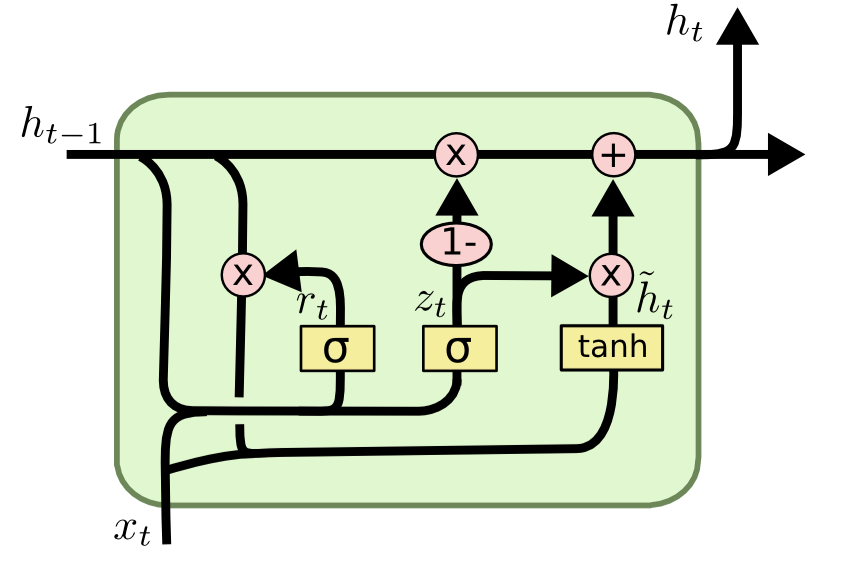
\includegraphics[width=0.5\textwidth]{img/LSTM3-var-GRU.png}
	\caption{Schemat komórki GRU.} Źródło: \cite{colah}.
	\label{fig:gru}
\end{figure}

Struktura komórki Gated Reccurent Unit (GRU) została wprowadzona w \cite{DBLP:journals/corr/ChoMGBSB14}. Komórka GRU w znacznym stopniu przypomina strukturę komórki LSTM. GRU również wykorzystuje bramki multiplikatywne do obliczania wartości stanu ukrytego w kolejnych krokach czasowych. Różnica polega na zastosowaniu dwóch bramek zamiast trzech, pełniących inne funkcje. Ciąg operacji realizowanych przez bramki i warstwy ukryte GRU omówiono poniżej.

Pierwsza bramka stosowana w ciągu przekształceń to reset gate, której aktywacje są obliczane jako:

\begin{equation}
	r_t = \sigma (W_r x_t + U_r h_{t-1})
\end{equation}

gdzie $W_r$ i $U_r$ są macierzami wag skojarzonymi z reset gate, $x$ oznacza wejście komórki a $h_{t-1}$ oznacza stan z poprzedniego kroku. Na podstawie $r$ obliczana jest wartość $\tilde{h_t}$:

\begin{equation}
	\tilde{h_t} = tanh(Wx_t + U(r_t \odot h_{t-1})
\end{equation}

gdzie $W$ i $U$ oznaczają skojarzone z operacją macierze wag, a $\tilde{h_t}$ oznacza kandydata do zastąpienia wektora stanu z poprzedniego kroku $h_{t-1}$. Intuicyjnie można powiedzieć, że reset gate ma za zadanie określić w jakich sytuacjach poprzedni stan sieci zawiera istotne informacje biorąc pod uwagę wejście w danym kroku. Jeśli $r_t$ będzie miało wartość bliską 0, $\tilde{h_t}$ będzie obliczone głównie na podstawie aktualnego wejścia $x_t$.

Ponadto wprowadza się update gate $z$ realizującą operacje:

\begin{equation}
	z_t = \sigma(W_z x_t + U_z h_{t-1})
\end{equation}

gdzie $W_z$ i $U_z$ to wagi skojarzone z update gate. Update gate jest wykorzystywane do aktualizacji stanu ukrytego sieci:

\begin{equation}
	h_t = z_t \tilde{h_t} + (1 - z_t) h_{t-1}
\end{equation}


Update gate odpowiada za określanie w jakim stopniu stan ukryty sieci z poprzedniego kroku $h_{t-1}$ jest nadal aktualny. Informacja ta jest wykorzystywana również do określenia w jakim stopniu $\tilde{h_t}$ może zastąpić $h_{t-1}$. Jest to znacząca zmiana w porównaniu do LSTM, gdzie do określania aktualności poprzedniego stanu i wyliczonego w aktualnym kroku służyły dwie osobne bramki. Schemat komórki GRU został przedstawiony na rysunku \ref{fig:gru}. Teoretyczne aspekty podstawowych pojęć omawianych w pracy i wprowadzona notacja posłużą w kolejnym rozdziale do wprowadzenia architektury ReNet wraz ze omówieniem wprowadzonej modyfikacji. 



\chapter{Problem badawczy}

W niniejszym rozdziale omówiono architekturę sieci ReNet i modyfikacje jakie zostały wprowadzone.

\section{ReNet}

\begin{figure}
\centering
	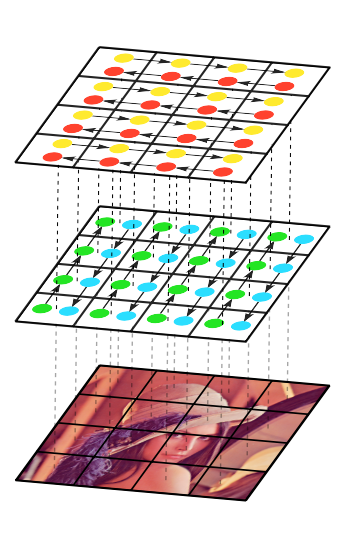
\includegraphics[width=0.5\textwidth]{img/ReNet.png}
	\caption{Schemat działania warstwy sieci ReNet.} Źródło: \cite{DBLP:journals/corr/VisinKCMCB15}.
	\label{fig:ReNet-single-layer}
\end{figure}

Sieci ReNet \cite{DBLP:journals/corr/VisinKCMCB15} są alternatywą dla sieci konwolucyjnych w zadaniu rozpoznawania obrazów. Warstwy konwolucyjne realizują operację nakładania filtrów na tensor wejściowy, przez co informacje na wyjściu warstwy mają charakter lokalny. Warstwa konwolucyjna w normalnym przypadku nie jest w stanie wykorzystać informacji zawartej w całym obrazie. ReNet jest sposobem na zaadresowanie tej kwestii poprzez wykorzystanie sieci rekurencyjnej do obliczania aktywacji warstwy sieci z wykorzystaniem informacji zawartej w całym obrazie.

Każda warstwa ReNet składa się z czterech sieci rekurencyjnych, które skanują obraz w czterech kierunkach: z góry na dół, od dołu do góry, z lewej do prawej oraz z prawej do lewej (Rysunek \ref{fig:ReNet-single-layer}). Wejściem każdej z sieci jest zbiór pikseli o niewielkich rozmiarach rozmiarach (ang. patch). W każdym kroku aktywacja warstwy ReNet jest obliczana na podstawie poprzedniego stanu sieci i aktualnie analizowanego zbioru pikseli. 

Obraz wejściowy można zdefiniować jako:

\begin{equation}
	X = \{x_{i,j}\},\qquad X \in \mathbb{R}^{w \textrm{x} h \textrm{x} c}
\end{equation}

gdzie $w, h$ to rozmiary obrazu, a $c$ to liczba kanałów dla każdego piksela obrazu. Liczbę patchy w pojedynczym wierszu i kolumnie obrazu wejściowego można zatem zapisać jako:

\begin{gather}
	I=\frac{w}{w_p} \\
	J=\frac{h}{h_p} \nonumber
\end{gather}

gdzie $w_p$ i $h_p$ to wysokość i szerokość patha. Zbiór wszystkich patchy obrazu wejściowego jest dany jako: $P = \{p_{i,j}\}, P \in \mathbb{R}^{w_p \textrm{x} h_p \textrm{x} c}$. Pionowe przejście sieci po wszystkich patchach obrazu można zapisać jako funkcję aktualnego patcha i aktywacji poprzedniego patcha:

\begin{gather}
    v_{i,j}^{F} = f_{VFWD} (v_{i,j-1}^F, p_{i,j}), \\
    v_{i,j}^{R} = f_{VREV} (v_{i,j+1}^R, p_{i,j}), \nonumber
\end{gather}

gdzie $f_{VFWD} (v_{i,j-1}^F, p_{i,j})$ to aktywacja sieci rekurencyjnej lub aktywacja komórki LSTM lub GRU. Wyjście po przejściu pionowym stanowi tensor $V = \{v_{i,j}\}_{i=1,...,I}^{j=1,...,J}$, będący mapą cech. Każdy element wyjścia $v_{i,j} \in \mathbb{R}^{2d}$ stanowi konkatenację aktywacji przejścia z góry na dół i z dołu na górę, gdzie $d$ to liczba jednostek rekurencyjnych wykorzystanych dla jednego patcha. Tensor $V$ jest wejściem dla drugiego elementu warstwy sieci realizującego przejście poziome. Operacja przejścia poziomego jest zdefiniowana analogicznie przez obliczenie aktywacji $f_{HFWD}, f_{HREV}$. Wynikiem tej operacji jest tensor $H = \{h_{i,j}\}$. 

Ostatecznie przekształcenie $\Phi$ realizowane przez całą warstwę sieci ReNet może zostać zapisane z wykorzystaniem wprowadzonych oznaczeń jako:

\begin{equation}
	\Phi: X \rightarrow V \rightarrow H
\end{equation}

\begin{figure}
\centering
	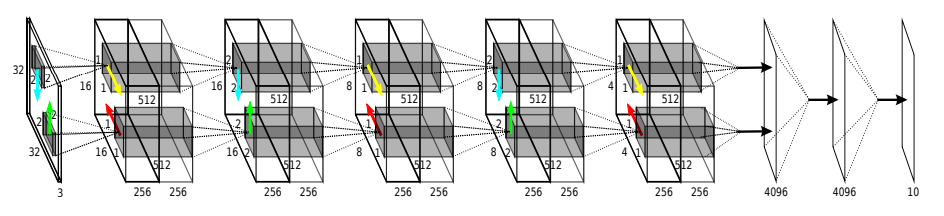
\includegraphics[width=0.9\textwidth]{img/ReNetArch.png}
	\caption{Schemat przepływu informacji w sieci ReNet.} Model ten został wykorzystany przez twórców architektury dla zbioru SVHN. Powyższy schemat przedstawia sieć z trzema warstwami ReNet, dwoma w pełni połączonymi warstwami oraz warstwą softmax. Obliczenia przeprowadzane w warstwie ReNet składają się z dwóch etapów: sieci skanujących obraz w kierunku góra-dół, dół-góra oraz lewo-prawo, prawo-lewo. W zastosowanej sieci rozmiar patchy w każdej warstwie wynosi 2x2. Warto zauważyć, że rozmiar patchy przy skanowaniu sieci w kierunku poziomym musi wynosić 1x1, aby aktwacje obliczane przy przejściu poziomym dotyczyły tej samej części obrazu co przy przejściu pionowym (w trakcie przejścia pionowego patch o rozmiarze 2x2xc zostaje zamieniony na aktywacje sieci 1x1x2d, gdzie d to liczba neuronów ukrytych w sieci rekurencyjnej - w tym wypadku d = 256). Aktywacje neuronów ukrytych są łączone dla przejść w przeciwnych kierunkach, więc wyjście po dwóch przejściach jest tensorem o rozmiarach $I,J,2d$. W każdej warstwie następuje zmniejszenie wymiarów obrazu. Efektem jest brak konieczności stosowania poolingu po warstwie ReNet. Warstwy w pełni połączone zawierają 4096 neuronów i wykorzystują funkcję aktywacji ReLu. Źródło: \cite{DBLP:journals/corr/VisinKCMCB15}
	\label{fig:ReNet}
\end{figure}

Każda kolejna warstwa sieci ReNet korzysta z wyjścia poprzedniej warstwy. Schemat działania sieci dla przykładowego obrazu, wraz z omówieniem realizowanych operacji został przedstawiony na rysunku \ref{fig:ReNet}.

\section{Krzywe wypełniające przestrzeń}

\begin{figure}
\centering
	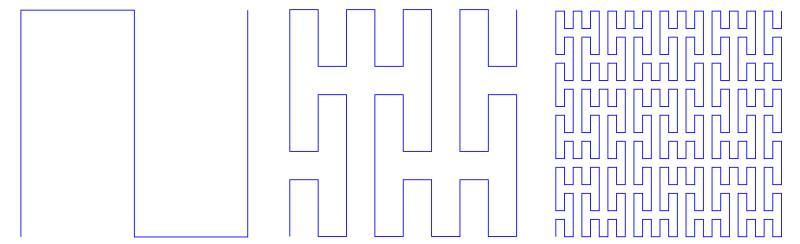
\includegraphics[width=0.9\textwidth]{img/peano_curve.png}
	\caption{Pierwsze trzy elementy ciągu tworzącego krzywą Peano.} Źródło: \cite{peano}.
	\label{fig:peano}
\end{figure}

Krzywe wypełniające przestrzeń to krzywe, które przedstawione na płaszczyźnie zawierają wszystkie punkty z kwadratu jednostkowego. W szczególności jeśli określimy krzywą wypełniającą jaką funkcję, która jest określona na przedziale jednostkowym $[0, 1]$, to krzywa wypełniająca przestrzeń będzie definiować mapowanie z przestrzeni dwuwymiarowej do jednowymiarowej i odwrotnie. 

Krzywa wypełniająca przestrzeń $\kappa$ może zostać określona określane przez rekurencyjny ciąg krzywych $k(n)$ ze zdefiniowanym pierwszym elementem $k(0)$ oraz sposobem konstruowania kolejnych:

\begin{equation}
	k(n+1) = f(k(n))
\end{equation}

$\kappa$ jest wtedy następującą granicą:

\begin{equation}
	\kappa = \lim_{n \rightarrow + \infty } k(n)
\end{equation}

\paragraph{Krzywa Hilberta}

\begin{figure}
\centering
	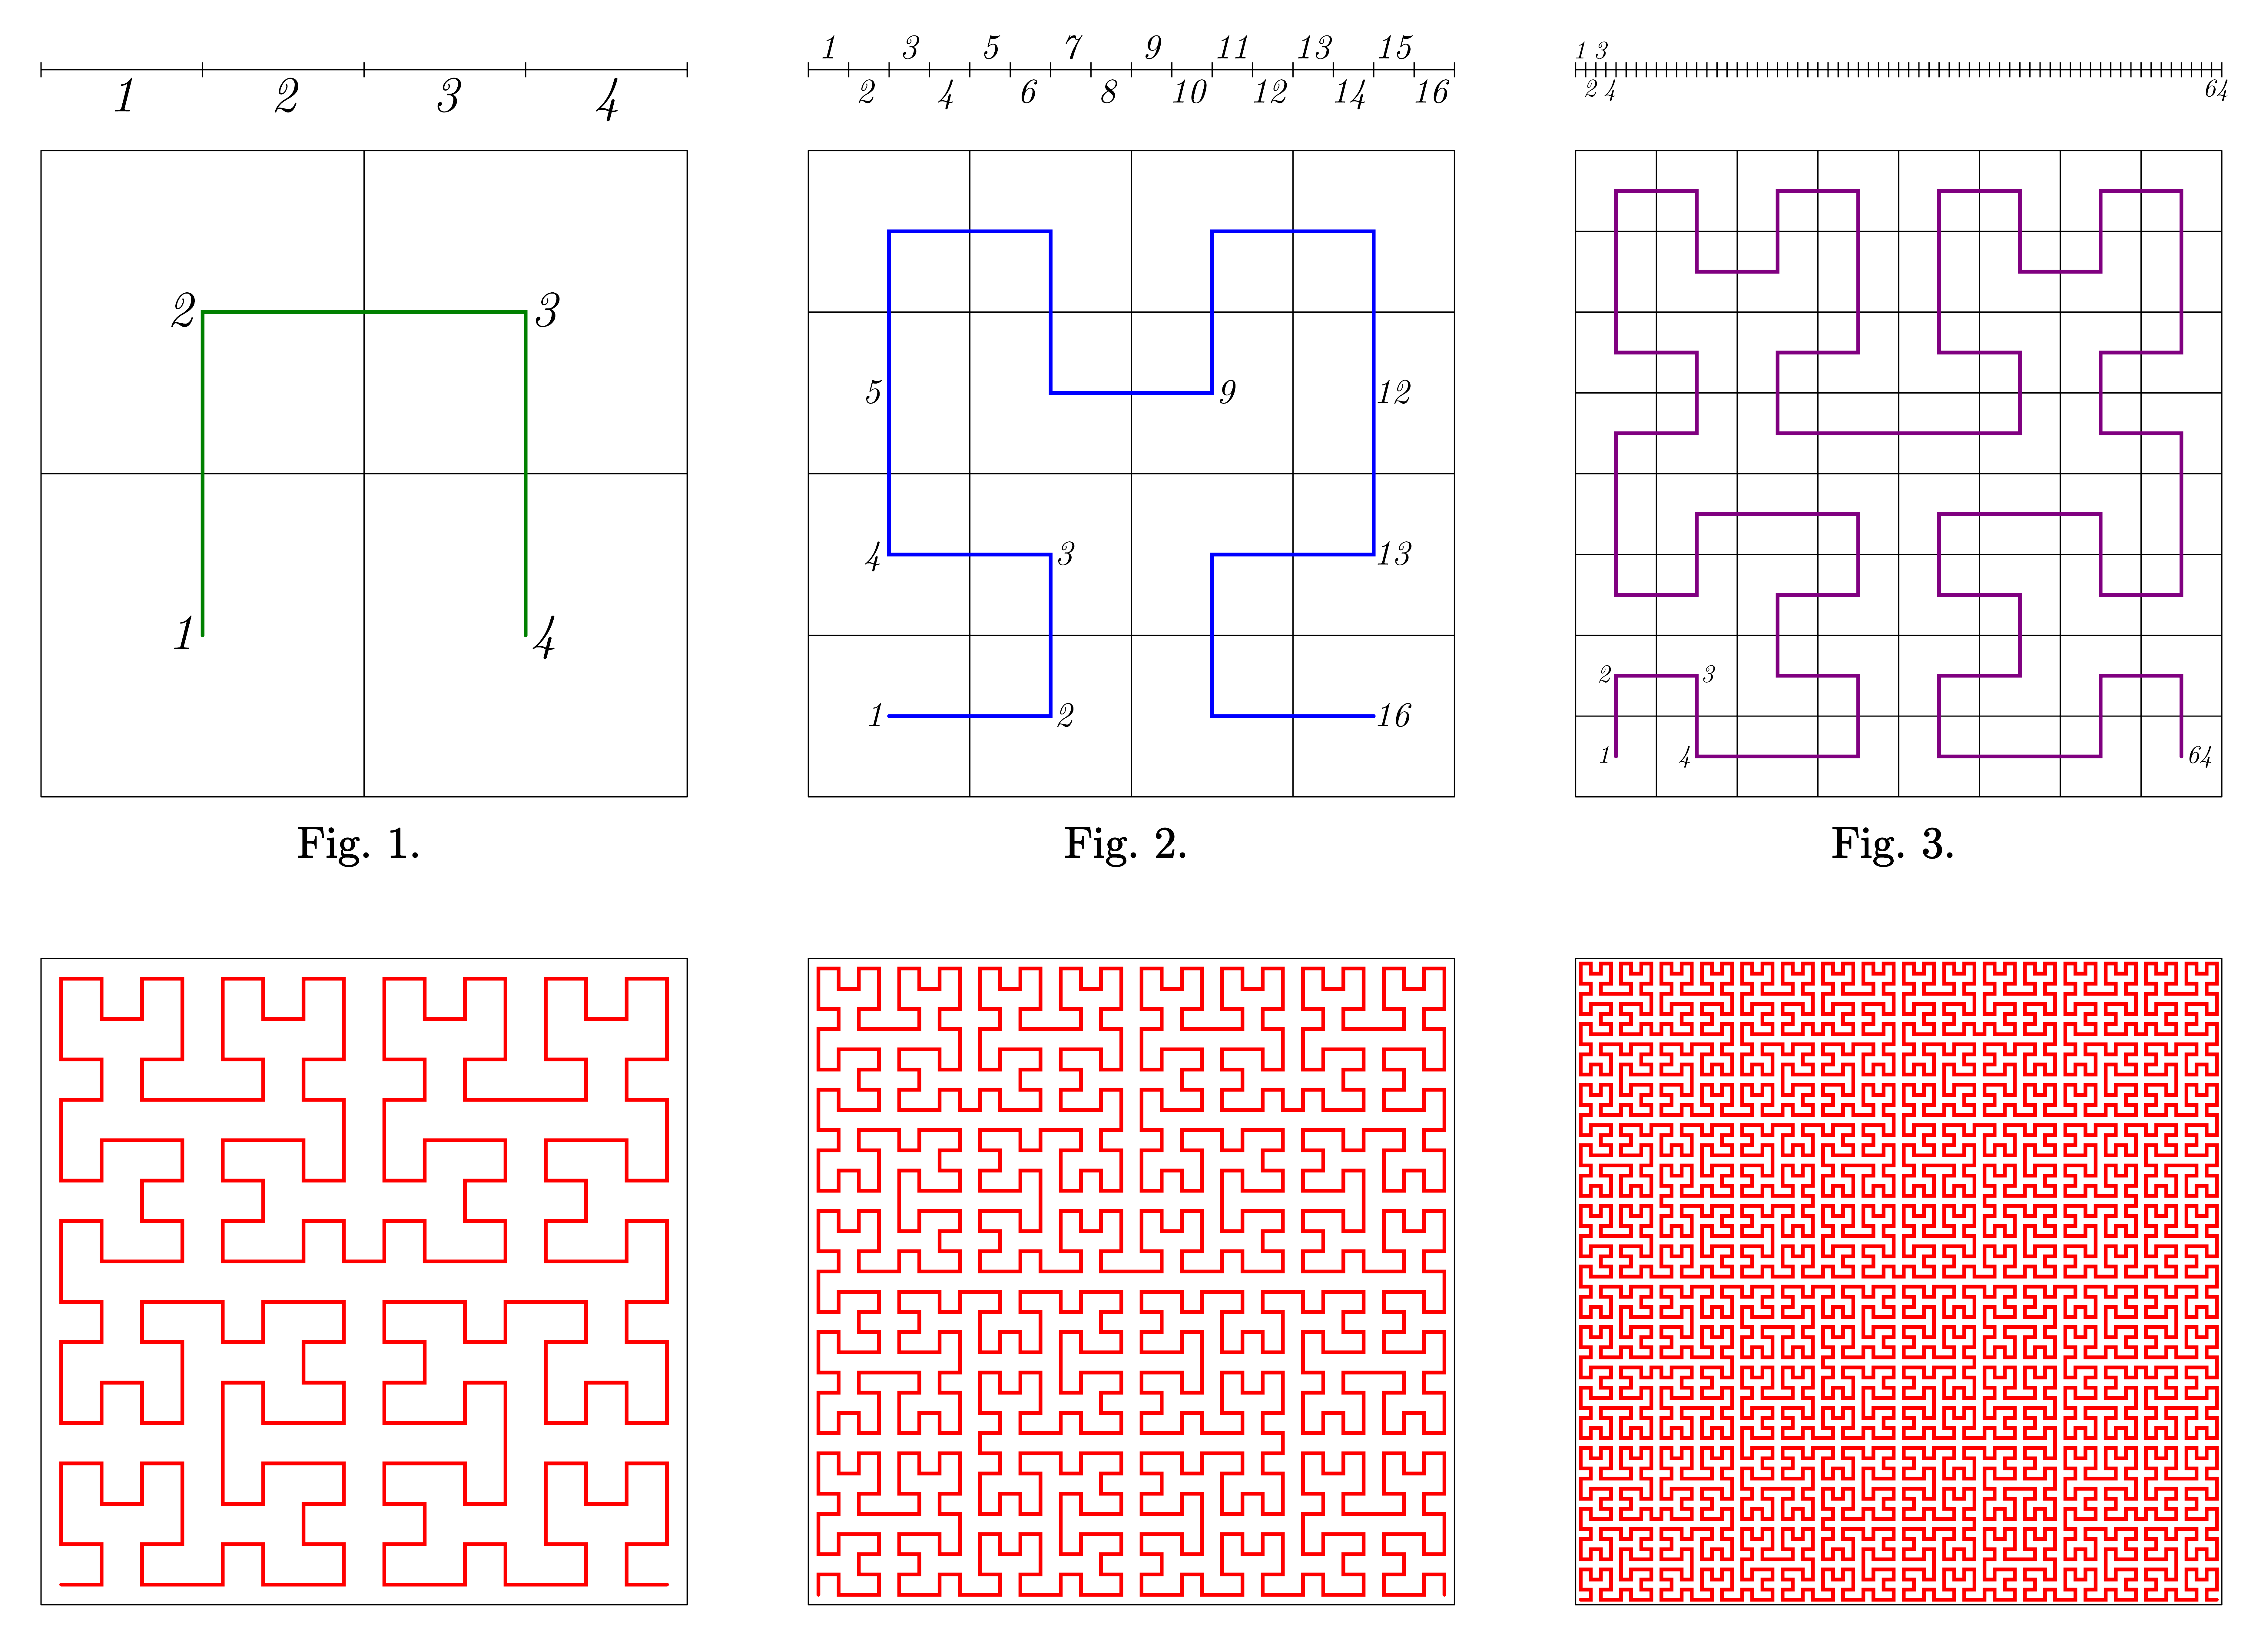
\includegraphics[width=1.0\textwidth]{img/hilbert_curve.png}
	\caption{Pierwsze sześć elementy ciągu tworzącego krzywą Hilberta.} Nad górnymi obrazkami zostały umieszczone punkty, do których zostałyby przypisane charakterystyczne punkty obrazu. Warto zwrócić uwagę, że dla krzywej stopnia pierwszego punkt 3 zostałby zmapowany w ten sam przedział odcinka co punkty 9, 10, 11 i 12 dla krzywej stopnia drugiego. Źródło: \cite{hilbert}.
	\label{fig:hilbert}
\end{figure}

Krzywa Hilberta $\mathcal{H}$ to krzywa wypełniająca przestrzeń posiadająca fraktalną strukturę. Pierwszy element ciągu tworzącego krzywą jest zdefiniowany jako trzy połączone odcinki rozmieszczone na bokach kwadratu. Kolejny element ciągu można uzyskać poprzez podział przestrzeni na 4 części i umieszczenie w każdej z części odpowiednio rotowanego poprzedniego elementu ciągu. Elementy w lewej górnej i prawej górnej części zostają umieszczone bez rotacji. Element w lewej dolnej części zostaje umieszczony po obrocie o 90$\degree$ w prawo, a element w prawej dolnej części zostaje umieszczony po obrocie o 90$\degree$ w lewo. Proces uzyskiwania kolejnych elementów krzywej został przedstawiony na rysunku \ref{fig:hilbert}.

Każdy z punktów będący końcem odcinka tworzącego krzywą Hilberta można przyjąć jako piksel obrazu. Korzystając z tego założenia krzywa Hilberta definiuje sposób przejścia po obrazie i zamianie współrzędnych dwuwymiarowych na jednowymiarowe.

Dodatkowo fraktalna struktura krzywej Hilberta powoduje, że odpowiednio wybrany fragment krzywej też jest krzywą Hilberta. Ta sama właściwość zachodzi dla elementu ciągu tworzącego krzywą, z tą różnicą, że wybrany fragment będzie poprzednim elementem ciągu. Fraktalna struktura powoduje również, że wraz ze wzrostem stopnia krzywej punkty znajdujące się w określonych częściach obrazu są mapowane do tych samych fragmentów krzywej. Własność ta została zademonstrowana na rysunku \ref{fig:hilbert}.

\section{Proponowana architektura sieci}

Modyfikacja architektury ReNet proponowana w tej pracy to wykorzystanie krzywej Hilberta do zmapowania punktów obrazu do przestrzeni jednowymiarowej, co można zapisać jako:

\begin{equation}
	x^{h} = \mathcal{H}(x)
\end{equation}

Aby uzyskać redukcję rozmiaru obrazu jak w oryginalnej ReNet i warstwach Poolingowych sieci konwolucyjnych wykorzystano podział na patche w analogiczny sposób do ReNet. W przypadku zmodyfikowanej ReNet zdefiniowano patche jako zbiór następujących po sobie pikseli po transformacji obrazu do jednego wymiaru: $P^{h} = \{ p_{i}^h \}$, $P^{h} \in \mathbb{R}^{w_p \textrm{x} c}$. Piksele należącego do tego samego patcha są traktowane jako jedno wejście sieci rekurencyjnej.

Zastąpiono cztery sieci rekurencyjne z warstwy ReNet dwiema sieciami rekurencyjnymi. Każda z sieci wykorzystuje wynik mapowania z dwóch wymiarów do jednego jako wejścia. Jedna z sieci przyjmuje wejścia w odwrotnej kolejności niż druga. Korzystając z notacji zdefiniowanej dla ReNet realizowane przekształcenie można zapisać jako:

\begin{gather}
	v_{i}^{F} = f_{FWD}(v_{i-1}^{F}, p_{i}^{h}) \\ \nonumber
	v_{i}^{R} = f_{REV}(v_{i+1}^{F}, p_{i}^{h})
\end{gather}

Wyjście sieci stanowi konkatenacja obliczonych aktywacji w obu kierunkach. Możliwe jest wykorzystanie patcha o rozmiarze 1. W tym przypadku sieć oblicza aktywacje jak dwukierunkowa sieć rekurencyjna.

Korzystając z fraktalnych właściwości krzywej Hilberta elementy obrazu po zmapowaniu i obliczeniu aktywacji sieci rekurencyjnych powinny nadal odpowiadać obszarom oryginalnych obrazów. Zastąpienie czterech sieci rekurencyjnych z architektury ReNet przez dwie może wpłynąć na czas trenowania sieci lub na zwiększoną elastyczność przy doborze struktury modelu. W przypadku gdy dla podobnej liczby warstw ReNet i zmodyfikowanej ReNet uzyskiwane wyniki klasyfikacji będą porównywalne oczekiwane jest skrócenie czasu trenowania. W przypadku gdy zmodyfikowana sieć ReNet będzie miała mniejsze zdolności do wytworzenia wartościowej reprezentacji, można zwiększyć jej możliwości przez dodanie dodatkowej warstwy z rozmiarem patcha 1. Istnieje możliwość dodania warstwy sieci z ReNet z rozmiarem patcha (1,1), ale spowoduje to dodanie czterech sieci rekurencyjnych. Należy mieć na uwadze, że są to modele wymagające znaczących nakładów mocy obliczeniowej, więc zmniejszenie liczby sieci rekurencyjnych na warstwę powinno umożliwić bardziej precyzyjne dostosowanie modelu do rozwiązywanego problemu. Dysponując opisem modeli zastosowanych w pracy i teoretycznymi podstawami wprowadzonymi w dwóch minionych rozdziałach można przystąpić do opisu przeprowadzonych eksperymentów.


\chapter{Przeprowadzone badania}

Rozdział ten zawiera opis metodyki prowadzenia badań wraz z przyjętym planem. Zawarto w nim także wyniki reprodukcji wyników z  pracy wprowadzającej ReNet, opis zbiorów danych i procedurę doboru hiperparametrów modeli.

\section{Metodyka badań}
W niniejszej sekcji omówiono przyjęty podział badań, oraz omówiono metodologię badawczą przyjętą do ich zrealizowania.

\subsection{Plan badań}
Badania podzielono na trzy zasadnicze części. Pierwszą z nich stanowiła reprodukcja wyników z \cite{DBLP:journals/corr/VisinKCMCB15}. Druga część polegała na porównaniu sieci ReNet, zmodyfikowanej wersji ReNet oraz sieci konwolucyjnych. W \cite{DBLP:journals/corr/VisinKCMCB15} zawarto informacje o wpływie wykorzystanej sieci rekurencyjnej na jakość klasyfikacji ReNet. W trzeciej części badań planowano zbadać wpływ wykorzystanej sieci rekurencyjnej na zmodyfikowaną wersję ReNet.

\subsection{Przyjęte metryki i sposób uczenia sieci}
W celu porównania jakości klasyfikacji porównano skuteczność klasyfikacji (accuracy), osiąganą na zbiorze testowym. W celu zredukowania wpływu wariancji estymatora na uzyskane wyniki zastosowano pięciokrotny sprawdzian krzyżowy. Każdy z algorytmów dysponował tymi samymi foldami jako zbiory testowe. 

Modele trenowano przez 50 epok, z rozmiarem batchy 32. Jako funkcję strat przyjęto entropię krzyżową. W trakcie uczenia monitorowano wartość funkcji start na zbiorze testowym i przerywano uczenie w momencie wystąpienia overfitingu, zgodnie z algorytmem w \cite{Goodfellow-et-al-2016}. Po wystąpieniu overfittingu i przerwaniu uczenia przywracano wagi dla modelu osiągającego najniższą odnotowaną wartość funkcji strat. Zmniejszano współczynnik uczenia po 5 epokach bez poprawy wartości funkcji strat dla zbioru testowego. Porównano wyniki osiągane dla trzech algorytmów uczenia: SGD, RMSprop oraz Adam. Najlepsze rezultaty osiągnięto dla algorytmu Adam, przez co został on wybrany jako algorytm optymalizacji we wszystkich eksperymentach.

\section{Reprodukcja wcześniejszych badań}

Pierwszym eksperymentem jaki wykonano było zreprodukowanie wyników z \cite{DBLP:journals/corr/VisinKCMCB15}. Celem reprodukcji było sprawdzenie poprawności przygotowanej implementacji ReNet. Wykorzystano zbiory MNIST, CIFAR10 oraz SVHN \cite{svhn}. W niniejszej sekcji podano krótki opis stosowanej metodyki i uzyskane wyniki.

\subsection{Statystyczna ewaluacja wyników}

Reprodukcja badań nie stanowi zasadniczej części badań. Z tego względu uproszczono proces zbierania wyników. Podane rezultaty są wynikiem pojedynczego procesu uczenia, bez powtarzania prób. W \cite{tom-mitchell-machine-learning} podano metody analizy błędu pojedynczego pomiaru skuteczności algorytmu.

Chcemy oszacować rzeczywisty błąd $err_{\mathcal{D}}$ popełniany przy przez hipotezę $h$ dla dowolonej próbki z rozkładu generującego dane $\mathcal{D}$ (ang. datagenerating distribution). W przypadku gdy $\mathcal{D}$ nie jest znane dysponujemy zbiorem danych $d$ wylosowanym z $\mathcal{D}$. Błąd popełniony przez $h$ na datasetcie $d$ dany jest wzorem:

\begin{equation}
	err_d = \frac{t}{n}
\end{equation}

gdzie $t$ to liczba błędnie zaklasyfikowanych przykładów z $n$ wszystkich przykładów w zbiorze $d$.
Przy założeniu, że $d$ zawiera próbki niezależne od siebie i $n$ jest większe od 30, $err_d$ jest najlepszym estymatorem $err_{\mathcal{D}}$. Przedział w którym wartość $err_{\mathcal{D}}$ znajduję się z prawdopodobieństwem około 95\% można wyznaczyć jako:

\begin{equation}
	err_{d} \pm 1.96 \sqrt{\frac{err_{d}(1 - err_{d})}{n}} 
\end{equation}

Przedziały te zostały podane wraz z uzyskanymi w trakcie reprodukcji badań wartościami skuteczności na zbiorze testowym.

\subsection{Wyniki reprodukcji}

\begin{table}
\centering
\caption{Wyniki reprodukcji wcześniejszych badań}
\label{tab:reproduction}
\begin{tabular}{ |c|c|c|c| } 
 \hline
 zbiór danych & \specialcell{błąd uzyskany\\ we wcześniejszej pracy} & \specialcell{błąd uzyskany\\ dla przygotowanej implementacji} & \specialcell{przedział ufności} \\ 
 \hline
 \makecell{mnist} & 0.0045 & 0.0628 & (0.0675, 0.0580) \\ 
 \hline
 \makecell{cifar10} & 0.1235 & 0.3787 & (0.3882, 0.3691) \\ 
 \hline
 \makecell{svhn} & 0.0238 & 0.5602 & (0.5662, 0.5541) \\ 
 \hline
\end{tabular}
\end{table}

Wynik reprodukcji został przedstawiony w tabeli \ref{tab:reproduction}. Można z łatwością zauważyć, że wartości accuracy uzyskanej przez twórców architektury ReNet są lepsze niż wyniki uzyskane dla przygotowanej implementacji. Żaden z wcześniej uzyskanych wyników nie mieści się przedziale ufności błędu obecnej implementacji.

Szczególnie niepokojące mogą być wartości błędu dla zbiorów cifar10 oraz svhn. W przypadku drugiego datasetu jest to związane z przerwaniem obliczeń po 5 epokach ze względu na brak pamięci. Model stosowany przy obecnej implementacji dla svhn wymagał wiele pamięci i jego trenowanie przebiegało niezwykle wolno. Czas uczenia jednej epoki wynosił  ponad godzinę. Zaobserwowano znaczący spadek czasu uczenia sieci przy wykorzystaniu RMSprop jak algorytmu optymalizacji. Zastosowanie w tym przypadku RMSprop wpłynęłoby na uzyskane wyniki, jednocześnie znacznie podważając wartość reprodukcji. Przyczyną znacząco gorszych wyników uzyskanych dla cifar10 i svhn może być także niewystarczająco dokładny dobór hiperparametrów sieci. Twórcy ReNet nie podali hiperparametrów takich jak współczynnik uczenia, czy prawdopodobieństwo wykluczenia neuronu w warstwie Dropout stosowanych w ich eksperymentach, co w tym przypadku znacząco utrudnia reprodukcję.

W związku z uzyskanymi rezultatami nasuwa się pytanie czy przygotowana implementacja sieci ReNet jest błędna? W tym momencie warto zwrócić uwagę na bardzo zbliżone wyniki oryginalnych badań i reprodukcji uzyskane dla datasetu mnist. Dodatkowo wyżej wymienione przypuszczalne powody słabych wyników nie muszą wskazywać na występowanie błędu w implementacji. 

\subsection{Testowanie poprawności implementacji}

Przeprowadzono dodatkową weryfikację poprawności implementacji ReNet przed przystąpieniem do dalszej pracy. Aby przeprowadzić test, należy wykorzystać możliwość ustawiania wag sieci rekurencyjnych zawartych w warstwie ReNet. Przy odpowiednio dobranych wartościach wag i funkcjach aktywacji sieć LSTM może działać jak mapowanie identycznościowe w każdym kroku czasowym. Oznacza to, że w każdym kroku czasowym wyjście sieci  będzie aktualną wartość wejścia. Dla wcześniej przyjętej parametryzacji LSTM można przyjąć wartości wag:

\begin{align*}
	W_f &= \bb{0} \\
	W_i &= \bb{0} \\
	W_c &= [\bb{0},I] \\
	W_o &= \bb{0}
\end{align*}

gdzie $\bb{0}$ oznacza macierz zerową, a $I$ macierz jednostkową.

Następnie należy zastąpić funkcję aktywacji $tanh$ przez funkcję identycznościową $f(x) = x$, funkcje aktywacji dla bramki forget przez funkcję stałą $f(x) = 0$ oraz funkcje aktywacji dla bramek input i output gate przez funkcję stałą $f(x) = 1$. W zależności od stosowanej implementacji sieci LSTM może posiadać inną parametryzację. Mimo tego metodą prób i błędów można zaleźć konfigurację wag i funkcji aktywacji, która powoduje działanie LSTM jako funkcji identycznościowej w każdym kroku czasowym. Dzięki tak skonfigurowanej sieci LSTM, można zapisać ciąg przekształceń realizowanych przez warstwę ReNet i sprawdzić czy dla przygotowanych danych wejściowych uzyskano odpowiednie wartości na wyjściu. Przygotowano testy opierające się na tej własności. Implementacja ReNet pomyślnie przeszła wszystkie  testy. Daje to mocne przesłanki aby uważać, że implementacja jest poprawna pomimo wyników reprodukcji.

\section{Opis eksperymentu}

W niniejszej sekcji przedstawiono szczegóły konfiguracji eksperymentu. Opisano wykorzystane zbiory danych, hardware, biblioteki oraz inne narzędzia. Dodatkowo omówiono przyjętą metodykę wyboru hiperparametrów modelu.

\subsection{Zbiory danych}

\begin{table}
\centering
\caption{Wykorzystane zbiory danych}
\label{tab:dataset}
\begin{tabular}{ |c|c|c|c|c|c| } 
 \hline
 nazwa zbioru & liczba obrazów & liczba klas & szerokość & wysokość & źródło \\ 
 \hline
 \makecell{Chest X-Ray\\ Images (Pneumonia)} & 5863 & 2 & $>$1500 & $>$1000 & \cite{xray-dataset}\\ 
 \hline
 \makecell{Flowers Recognition} & 4242 & 5 & 320 & 240 & \cite{flowers-dataset} \\ 
 \hline
 \makecell{Fashion MNIST} & 70000 & 10 & 28 & 28 & \cite{fashion-dataset} \\ 
 \hline
 \makecell{Natural Images} & 6899 & 8 & $>$200 & $>$50 & \cite{natural-img-dataset} \\ 
 \hline
\end{tabular}
\end{table}

Do przeprowadzenia eksperymentów wykorzystano datasety z różnych domen, mające przetestować zdolność badanych sieci do ekstrakcji istotnych cech z obrazów. Zestawienie wykorzystanych zbiorów przedstawiono w tabeli \ref{tab:dataset}. Wykorzystano datasety o różnej liczności i różnych rozmiarach obrazów oraz różnej liczbie klas.

Dla wszystkich datasetów zastosowano przesuwanie obrazów w poziomie o -2, 0 lub 2 piksele. Jest to procedura zastosowana w badaniach wprowadzających ReNet i ma na celu zredukowanie overfittingu. W przypadku datasetu Chest X-Ray dokonano konwersji do skali szarości, ponieważ głębia kolorów nie wnosiła wiele informacji w zdjęciach rentgenowskich. Wszystkie wejścia zostały znormalizowane do zerowej średniej i jednostkowej wariancji w celu ułatwienia optymalizacji modeli. W procesie przetwarzania wstępnego zmieniano rozmiar obrazów do 64x64 lub 32x32 pikseli. Dla przygotowanej implementacji sieci ReNet zatosowanej do obrazów o dużych rozmiarach model osiąga wielkość uniemożliwiającą trenowanie go na powszechnie dostępnych kartach graficznych. Daje to istotne ograniczenie obszaru zastosowań sieci ReNet i jednocześnie definiuje konieczny krok przetwarzania wstępnego obrazów przed rozpoczęciem procesu uczenia. Nie wszystkie zbiory uczące można poddać zmniejszeniu rozmiaru obrazu bez utraty informacji mających wpływ na klasyfikację.

Wykorzystane datasety są w różnym stopniu niezbalansowane. Problem ten rozwiązano przez zastosowanie undersamplingu zbioru treningowego do klasy zawierającej najmniejszą liczbę przykładów uczących. Rozwiązanie to zastosowano przy doborze hiperparametrów oraz przy sprawdzianie krzyżowym dla każdego foldu.

W trakcie poszukiwania zbiorów danych odnotowano znaczący spadek jakości klasyfikacji modeli ReNet dla datasetów zawierających dużo klas i mało przykładów uczących przypadających na pojedynczą klasę takich jak \cite{fruits-dataset} czy \cite{face-dataset}. Analiza problemu ReNet dla tej grupy zbiorów uczących wymaga głębszych badań i wnikliwej analizy problemu, jednakże nie jest to cel tej pracy. Z tego powodu wymienione datasety nie zostały wykorzystane w dalszych testach. 

\subsection{Wykorzystane narzędzia i hardware}

Znaczna część eksperymentów została przeprowadzona na platformie Google Colab oraz Google Cloud Platform z wykorzystaniem AI platform. Google Colab pozwala na wykorzystanie maszyn wirtualnych z GPU i TPU do realizacji projektów naukowych. Ze względu na dynamiczną alokację maszyn wirtualnych dla każdej sesji nie można określić jaki model karty graficznej bądź TPU został wykorzystany do obliczeń. Reprodukcja badań z \cite{DBLP:journals/corr/VisinKCMCB15} oraz pomiar czasu uczenia modeli zostały wykonane przy pomocy komputera z procesorem IntelCore i7 8700 i kartą graficzną GTX 1070Ti.

Implementacja analizowanych modeli została wykonana przy pomocy biblioteki keras \cite{keras} z backendem tensorflow \cite{tensorflow}. W badaniach wykorzystano także biblioteki scikit-learn \cite{scikit-learn} oraz numpy \cite{numpy}. Wszystkie datasety zostały pobrane z wykorzystaniem publicznego API seriwsu kaggle.

\subsection{Dobór struktury i hiperparametrów modelu}

Aby zapewnić najlepsze osiągi porównywanych algorytmów z uwzględnieniem ograniczonej mocy obliczeniowej dokonano doboru wybranych hiperparametrów modeli. Do zbioru optymalizowanych parametrów dla każdego datasetu zaliczały się:

\begin{itemize}
\item współczynik uczenia,
\item współczynnik regularyzacji wybranych warstw,
\item liczba warstw dokonujących ekstrakcji cech,
\item liczba warstw w pełni połączonych,
\item liczba neuronów w warstwach w dokonujących ekstrakcji cech,
\item liczba neuronów w warstwach w pełni połączonych,
\item współczynnik prawdopodobieństwa wykluczenia neuronu w procedurze dropout dla wybranych warstw.
\end{itemize}

Mając na uwadze ograniczenia dostępnej mocy obliczeniowej zdecydowano się wykorzystać zmodyfikowaną wersję alogorytmu Grid Search. Każdy z hiperparametrów dobierano osobno na podstawie przyjętego zakresu. Po wybraniu najlepszej wartości jednego z hiperparametrów dobierano wartość kolejnego. Modyfikacja ta polega na zastąpieniu przeszukiwania zupełnego przyjętej dyskretnej przestrzeni hiperparametrów przez przeszukiwania zachłanne. W sytuacji gdy dostępne zasoby obliczeniowe są ograniczone jest to sposób na uniknięcie wielu niepotrzebnych obliczeń. Warto zwrócić uwagę, że jest to podejście naiwne, ponieważ przyjęto założenie o niezależności wpływu kontrolowanych czynników na proces uczenia.

Modele uczono przez 20 epok porównując osiągane wyniki. Do dalszych testów wybrano modele osiągające największą skuteczność (accuracy) na zbiorze testowym. Dokładna procedura doboru hiperparametrów została opisana w postaci poniższego algorytmu:

\begin{algorithm}[H]
\SetAlgoLined
\caption{Procedura doboru hiperparametrów}
1. Dobór hiprametrów mających największy wpływ na proces uczenia i.e. parametrów mających wpływ na funckję strat - współczynnik uczenia oraz współczynniki reugraryzacji l1 i l2.\\
2. Dobór liczby warstw odpowiedzialnych za ekstrakcję cech (warstwy ReNet, zmodyfikowana ReNet lub konwolucyjne) wraz z prawdopodobieństwiem maskowania neuronu w warstwach Dropout.\\
3. Dobór liczby neuronów w warstwach odpowiedzialnych za ekstrakcję cech.\\
4. Dobór liczby neuronów w warstwach w pełni połączonych wraz z prawdopodobieństwem maskowania neuronu w warstwach Dropout.\\
\end{algorithm}

Warto zwrócić uwagę, że w punkcie 4 powyższej procedury przyjęto, że każdy model posiada dwie warstwy w pełni połączone. W celu porównania wybranych architektur, modele powinny dysponować taką samą liczbą warstw dokonujących klasyfikację na podstawie nauczonej reprezentacji. Badania nie mają na celu uzyskanie jak najlepszych możliwych modeli do rozwiązania wybranych problemów, a jedynie porównanie zdolności modeli do ekstrachowania odpowiednich cech z obrazów.

W punktach 2 i 4 dobór liczby warstw jest połączony z doborem współczynnika regularyzacji, ponieważ w niektórych przypadkach bardziej wskazane jest stosowanie głębszych modeli ze zwiększoną regularyzacją. Nie zmienia to naiwności opisywanej metody. Głębokość sieci i współczynniki regularyzacji to dwa czynniki, o których wiadomo, że są ze sobą powiązane. Możliwe jest występowanie innych powiązanych czynników, których wzajemna relacja nie została uwzględniona w powyższej procedurze. 

Przyjęto uproszczenie w punkcie 3. Dla sieci ReNet oraz ReNet z modyfikacją przyjęto tą samą liczbę neuronów w każdej warstwie. Takie samo rozwiązanie przyjęto w pracy wprowadzającej ReNet. Ograniczenie to pozwala zredukować liczbę poszukiwanych parametrów.

Dla parametrów odpowiadających za liczność neuronów w warstawach porówywano osiągane wyniki dla kolejnych potęg 2 z zakresu $[32, 4096]$. W przypadku współczynnika uczenia oraz współczynników reugraryzacji l1 i l2 sprawdzano parametry z zakresu $[10^{-2}, 10^{-8}]$ w skali logarytmicznej.

Opisana procedura pozwala na zmniejszenie nakładu obliczeniowego potrzebnego do wyboru modelu. Nie istnieje gwarancja, że otrzymany model jest optymalny w analizowanej przestrzeni, ale można liczyć, że będzie wystarczająco dobry do przeprowadzenia porównania.

\begin{figure}
\centering
	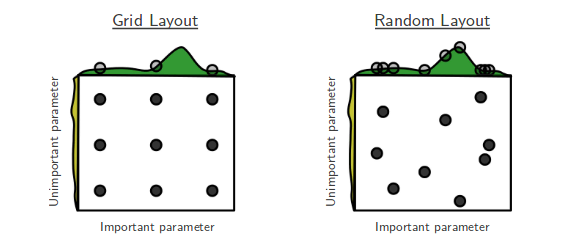
\includegraphics[width=0.8\textwidth]{img/grid_search.png}
	\caption{Porównanie Grid Search i Random Search.} Źródło: \cite{Bergstra:2012:RSH:2503308.2188395}.
	\label{fig:hyperparams}
\end{figure}

Inne dostępne rozwiązania problemu doboru hiperametrów to wykorzystanie algorytmów Grid Search lub Random Search. Grid Search nie jest zalecaną metodą. Często hiperparametry mają różny wpływ na wyniki procesu uczenia. Maksimum optymalizowanej metryki może występować pomiędzy punktami tworzonej siatki, jak to zostało przedstawione na rysunku \ref{fig:hyperparams}. W przypadku w którym jeden z hiperparametrów ma większy wpływ na osiągane wyniki należy zwiększyć liczbę przeszukiwanych punktów. Random Search unika tego problemu przez wybieranie losowych punktów z przestrzeni, przez co hiperparametry mające większy wpływ na proces uczenia są próbkowane w większej liczbie punktów i istnieje większa szansa na znalezienie efektywniejszej wartości. Wadą obu algorytmów jest duża liczba iteracji potrzebnych do przeszukania przestrzeni, rosnąca wraz ze wzrostem liczby hiperparametrów i brak wykorzystywania wcześniej zdobytych informacji do poprawy osiągniętego wyniku. W rozdziale tym przedstawiono stosowaną metodykę oraz narzędzia wykorzystane w przeprowadzonych eksperymentach. W kolejnym rozdziale zostaną przedstawione wyniki uzyskane zgodnie z metodyką opisaną w tym rozdziale.


\chapter{Wyniki}

W niniejszym rozdziale przedstawiono wyniki uzyskane zgodnie z przyjętą i wcześniej opisaną metodologią.

\section{Strukutra modeli i wartości hiperparametrów}

\begin{table}[ht]
\centering
\caption{Zestawienie struktury wykorzystanych modeli - współczynniki wpływające na funkcję strat}
\label{tab:hyperparams-coefs}
\begin{tabular}{ |c|c|c|c|c| } 
 \hline
 zbiór danych & algorytm & \makecell{współczynnik\\uczenia} & \makecell{współczynnik \\ reg. l1} & \makecell{współczynnik\\ reg. l2}  \\ 
 \hline
 \hline
 \multirow{3}{*}{\makecell{Chest X-Ray\\ Images (Pneumonia)}} &
 \multicolumn{1}{l}{ReNet} & \multicolumn{1}{l}{0.001} & \multicolumn{1}{l}{0.0000001} & \multicolumn{1}{l|}{0.000001} \\\cline{2-5} &
 \multicolumn{1}{l}{zmodyf. ReNet} & \multicolumn{1}{l}{0.001} & \multicolumn{1}{l}{0.0001} & \multicolumn{1}{l|}{0.001} \\\cline{2-5} &
 \multicolumn{1}{l}{conv} & \multicolumn{1}{l}{0.0001} & \multicolumn{1}{l}{0.0001} & \multicolumn{1}{l|}{0.00000001} \\\hline
 \hline
 \multirow{3}{*}{\makecell{Flowers Recognition}} & 
 \multicolumn{1}{l}{ReNet} & \multicolumn{1}{l}{0.001} & \multicolumn{1}{l}{0.00000001} & \multicolumn{1}{l|}{0.00000001} \\\cline{2-5} &
 \multicolumn{1}{l}{zmodyf. ReNet} & \multicolumn{1}{l}{0.001} & \multicolumn{1}{l}{0.00000001} & \multicolumn{1}{l|}{0.00000001} \\\cline{2-5} &
 \multicolumn{1}{l}{conv} & \multicolumn{1}{l}{0.001} & \multicolumn{1}{l}{0.00000001} & \multicolumn{1}{l|}{0.00000001} \\\hline
 \hline
 \multirow{3}{*}{\makecell{Fashion MNIST}} & 
 \multicolumn{1}{l}{ReNet} & \multicolumn{1}{l}{0.001} & \multicolumn{1}{l}{0.0000001} & \multicolumn{1}{l|}{0.0000001} \\\cline{2-5} &
 \multicolumn{1}{l}{zmodyf. ReNet} & \multicolumn{1}{l}{0.001} & \multicolumn{1}{l}{0.00001} & \multicolumn{1}{l|}{0.00001} \\\cline{2-5} &
 \multicolumn{1}{l}{conv} & \multicolumn{1}{l}{0.001} & \multicolumn{1}{l}{0.00000001} & \multicolumn{1}{l|}{0.00000001} \\\hline
 \hline
 \multirow{3}{*}{\makecell{Natural Images}} & 
 \multicolumn{1}{l}{ReNet} & \multicolumn{1}{l}{0.001} & \multicolumn{1}{l}{0.00000001} & \multicolumn{1}{l|}{0.00000001} \\\cline{2-5} &
 \multicolumn{1}{l}{zmodyf. ReNet} & \multicolumn{1}{l}{0.001} & \multicolumn{1}{l}{0.000000001} & \multicolumn{1}{l|}{0.000000001} \\\cline{2-5} &
 \multicolumn{1}{l}{conv} & \multicolumn{1}{l}{0.001} & \multicolumn{1}{l}{0.00000001} & \multicolumn{1}{l|}{0.00000001} \\\hline
\end{tabular}
\end{table}

\begin{table}
\centering
\addtolength{\leftskip} {-2cm}
\addtolength{\rightskip}{-2cm}
\caption{Zestawienie struktury wykorzystanych modeli - część odpowiedzialna za ekstrakcję cech}
\label{tab:hyperparams-extraction}
\begin{tabular}{ |c|c|c|c|c|c| } 
 \hline
 zbiór danych & algorytm & \makecell{l. warstw\\ ekstrakcji} & \makecell{l. neuronów\\ w warstwach\\ ekstrakcji} & \makecell{rozm. patchy/\\ rozmiar filtrów} & dropout \\ 
 \hline
 \hline
 \multirow{3}{*}{\makecell{Chest X-Ray\\ Images (Pneumonia)}} &
 \multicolumn{1}{l}{ReNet} & \multicolumn{1}{l}{3} & \multicolumn{1}{l}{256} & \multicolumn{1}{l}{(2,2)-(2,2)-(2,2)} & \multicolumn{1}{l|}{0.1} \\\cline{2-6} &
 \multicolumn{1}{l}{zmodyf. ReNet} & \multicolumn{1}{l}{3} & \multicolumn{1}{l}{256} & \multicolumn{1}{l}{4-4-4} & \multicolumn{1}{l|}{0.1} \\\cline{2-6} &
 \multicolumn{1}{l}{conv} & \multicolumn{1}{l}{3} & \multicolumn{1}{l}{32-64-128} & \multicolumn{1}{l}{(4,4)-(2,2)-(2,2)} & \multicolumn{1}{l|}{-} \\\hline
 \hline
 \multirow{3}{*}{\makecell{Flowers Recognition}} & 
 \multicolumn{1}{l}{ReNet} & \multicolumn{1}{l}{3} & \multicolumn{1}{l}{256} & \multicolumn{1}{l}{(2,2)-(2,2)-(2,2)} & \multicolumn{1}{l|}{0.1} \\\cline{2-6} &
 \multicolumn{1}{l}{zmodyf. ReNet} & \multicolumn{1}{l}{3} & \multicolumn{1}{l}{256} & \multicolumn{1}{l}{4-4-4} & \multicolumn{1}{l|}{0.2} \\\cline{2-6} &
 \multicolumn{1}{l}{conv} & \multicolumn{1}{l}{4} & \multicolumn{1}{l}{128-128-256-512} & \multicolumn{1}{l}{(4,4)-(4,4)-(2,2)-(2,2)} & \multicolumn{1}{l|}{-} \\\hline
 \hline
 \multirow{3}{*}{\makecell{Fashion MNIST}} & 
 \multicolumn{1}{l}{ReNet} & \multicolumn{1}{l}{2} & \multicolumn{1}{l}{256} & \multicolumn{1}{l}{(2,2)-(2,2)} & \multicolumn{1}{l|}{0.1} \\\cline{2-6} &
 \multicolumn{1}{l}{zmodyf. ReNet} & \multicolumn{1}{l}{3} & \multicolumn{1}{l}{256} & \multicolumn{1}{l}{4-4-4} & \multicolumn{1}{l|}{0.1} \\\cline{2-6} &
 \multicolumn{1}{l}{conv} & \multicolumn{1}{l}{5} & \multicolumn{1}{l}{32-32-64-64-128} & \multicolumn{1}{l}{(4,4)-(4,4)-(2,2)-(2,2)-(2,2)} & \multicolumn{1}{l|}{-} \\\hline
 \hline
 \multirow{3}{*}{\makecell{Natural Images}} & 
 \multicolumn{1}{l}{ReNet} & \multicolumn{1}{l}{2} & \multicolumn{1}{l}{128} & \multicolumn{1}{l}{(2,2)-(2,2)} & \multicolumn{1}{l|}{0.1} \\\cline{2-6} &
 \multicolumn{1}{l}{zmodyf. ReNet} & \multicolumn{1}{l}{7} & \multicolumn{1}{l}{128} & \multicolumn{1}{l}{4-4-4-4-4-4-4} & \multicolumn{1}{l|}{0.1} \\\cline{2-6} &
 \multicolumn{1}{l}{conv} & \multicolumn{1}{l}{3} & \multicolumn{1}{l}{64-128-256} & \multicolumn{1}{l}{(4,4)-(2,2)-(2,2)} & \multicolumn{1}{l|}{-} \\\hline
\end{tabular}
\end{table}


\begin{table}[ht]
\centering
\caption{Struktura wykorzystanych modeli - część odpowiedzialna za klasyfikację}
\label{tab:hyperparams-classification}
\begin{tabular}{ |c|c|c|c| } 
 \hline
  zbiór danych & algorytm & \makecell{l. neuronów\\ w warstwach\\ klasyfikacji} & dropout  \\ 
 \hline
 \hline
 \multirow{3}{*}{\makecell{Chest X-Ray\\ Images (Pneumonia)}} &
 \multicolumn{1}{l}{ReNet} & \multicolumn{1}{l}{512} & \multicolumn{1}{l|}{0.1} \\\cline{2-4} &
 \multicolumn{1}{l}{zmodyf. ReNet} & \multicolumn{1}{l}{512} & \multicolumn{1}{l|}{0.1} \\\cline{2-4} &
 \multicolumn{1}{l}{conv} & \multicolumn{1}{l}{512} & \multicolumn{1}{l|}{0.5} \\\hline
 \hline
 \multirow{3}{*}{\makecell{Flowers Recognition}} & 
 \multicolumn{1}{l}{ReNet} & \multicolumn{1}{l}{4096} & \multicolumn{1}{l|}{0.1} \\\cline{2-4} &
 \multicolumn{1}{l}{zmodyf. ReNet} & \multicolumn{1}{l}{1024} & \multicolumn{1}{l|}{0.1} \\\cline{2-4} &
 \multicolumn{1}{l}{conv} & \multicolumn{1}{l}{1024} & \multicolumn{1}{l|}{0.5} \\\hline
 \hline
 \multirow{3}{*}{\makecell{Fashion MNIST}} & 
 \multicolumn{1}{l}{ReNet} & \multicolumn{1}{l}{4096} & \multicolumn{1}{l|}{0.1} \\\cline{2-4} &
 \multicolumn{1}{l}{zmodyf. ReNet} & \multicolumn{1}{l}{512} & \multicolumn{1}{l|}{0.1} \\\cline{2-4} &
 \multicolumn{1}{l}{conv} & \multicolumn{1}{l}{1024} & \multicolumn{1}{l|}{0.7} \\\hline
 \hline
 \multirow{3}{*}{\makecell{Natural Images}} & 
 \multicolumn{1}{l}{ReNet} & \multicolumn{1}{l}{4096} & \multicolumn{1}{l|}{0.1} \\\cline{2-4} &
 \multicolumn{1}{l}{zmodyf. ReNet} & \multicolumn{1}{l}{256} & \multicolumn{1}{l|}{0.1} \\\cline{2-4} &
 \multicolumn{1}{l}{conv} & \multicolumn{1}{l}{1024} & \multicolumn{1}{l|}{0.5} \\\hline
\end{tabular}
\end{table}

Wybrane parametry modeli, uzyskane we wcześniej opisanym procesie doboru hiperparametrów zostały przedstawione w tabelach \ref{tab:hyperparams-coefs}, \ref{tab:hyperparams-extraction}, oraz \ref{tab:hyperparams-classification}.

Z przedstawionych tabel można wywnioskować kilka właściwości zastosowanych modeli. Pierwszym faktem, na który warto zwrócić uwagę to regularyzacja wykorzystana w procesie uczenia.
Dla wszystkich sieci współczynniki regularyzacji l1 były aplikowane do aktywacji pierwszej warstwy w pełni połączonej z funkcją aktywacji ReLu, a regularyzacja l2 została zaaplikowana do wag ostatniej warstwy połączonej z funkcją aktywacji softmax. Dla sieci ReNet współczynniki te są niekiedy wyższe niż dla sieci konwolucyjnych, jednakże w przypadku sieci konolucyjnych regularyzacja l2 została zaaplikowana również do warstw konwolucyjnych.
W tabeli \ref{tab:hyperparams-extraction} można zauważyć niskie wartości dropoutu zaaplikowanego do warstw ReNet. Dla wyższych wartości odnotowano znaczący spadek wartości metryk. W przypadku warstw konwolucyjnych zastosowano Batch Normalization zamiast dropoutu. Normalizacja ta występowała w sieci bezpośrednio po zaaplikowaniu nieliniowości (funkcji aktywacji) do aktywacji warstwy konwolucyjnej lub po zaaplikowaniu nieliniowości i MaxPoolingu. Zaaplikowanie Bartch Normalization do sieci ReNet skutkowało znacznym obniżeniem wartości obserwowanych metryk. 
Dodatkowo można porównać wysokie współczynniki regularyzacji dropout dla sieci konwolucyjnych w tabeli \ref{tab:hyperparams-classification} z niskimi wartościami dla sieci ReNet. Na podstawie danych z tabeli \ref{tab:hyperparams-classification} można zauważyć, że ReNet wymagało znacznie większej liczby neuronów w warstwie w pełni połączonej niż inne architektury.

Powodem uzyskania takich wartości jest różna zdolność modeli do uczenia się. W procesie uczenia na tych samych danych sieci ReNet znajdowały się często w reżimie niedouczenia. W przypadku sieci konwolucyjnych zastosowane techniki regularyzacji pozwalały uniknąć przeuczenia sieci. Można wnioskować, że dla wykorzystanych datasetów modele ReNet wykazują mniejsze capacity niż sieci konwolucyjne.

Dla zbioru Natural Images wykorzystano znacznie głębszą architekturę modelu sieci ReNet z modyfikacją niż dla dwóch pozostałych modeli. Sieć ta miała problemy z nauczeniem się tego datasetu. Nie udało się ustalić powodu tego problemu.

\section{Porównanie skuteczności modeli}

\begin{table}[ht]
    \centering
    \caption{Uśrednione wyniki sprawdzianu krzyżowego dla 5 foldów}
    \begin{tabular}{|r|l|l|l|}
  \hline
    & ReNet & modif ReNet & conv \\
  \hline
  \makecell{Chest X-Ray\\ Images (Pneumonia)} & 0.91 & 0.93 & 0.94 \\
  \hline
  \makecell{Flowers Recognition} & 0.53 & 0.55 & 0.65 \\
  \hline
  \makecell{Fashion MNIST} & 0.86 & 0.0 & 0.0 \\
  \hline
  \makecell{Natural Images} & 0.84 & 0.75 & 0.93 \\
  \hline
\end{tabular}

    \label{table:cross_validation}
\end{table}

\begin{table}[ht]
    \centering
    \caption{Porównanie osiągniętych p-wartości oraz H-wartości dla testu Kruskala-Wallisa dokładności modeli}
    \begin{tabular}{|r|l|l|}
  \hline
  zbiór danych & wartość statystyki H & p-wartość \\
  \hline
  \makecell{Chest X-Ray\\ Images (Pneumonia)} & 11.579 & 0.003 \\
  \hline
  \makecell{Flowers Recognition} & 10.220 & 0.006 \\
  \hline
  \makecell{Fashion MNIST} & 10.820 & 0.004 \\
  \hline
  \makecell{Natural Images} & 12.5 & 0.001 \\
  \hline
\end{tabular}

    \label{table:kruskal}
\end{table}

\begin{table}[ht]
    \centering
    \caption{Zestawienie osiągniętych p-wartości dla testów post-hoc}
    \begin{tabular}{|r|l|l|l|}
  \hline
  dataset & ReNet vs modif ReNet & ReNet vs conv & modif ReNet vs conv \\
  \hline
  \makecell{Chest X-Ray\\ Images (Pneumonia)} & 0.016 & 0.001 & 0.001 \\
  \hline
  \makecell{Flowers Recognition} & 0.189 & 0.001 & 0.001 \\
  \hline
  \makecell{Fashion MNIST} & 0.036 & 0.001 & 0.000 \\
  \hline
  \makecell{Natural Images} & 0.001 & 0.001 & 0.001 \\
  \hline
\end{tabular}

    \label{table:posthoc}
\end{table}

W pierwotnym projekcie eksperymentów zakładano wykorzystanie testu Friedmanna z testami post-hoc Nemenyiego. Test Friedmana wymaga zebrania wyników dla co najmniej 6 datasetów. Ze względu na ograniczenia czasowe nie udało się zebrać tylu wyników. Podjęto decyzję o przeanalizowaniu efektywności modeli dla każdego datasetu osobno. Testy na normalność rozkładu tracą moc wraz ze spadkiem liczby próbek. Po sprawdzianie krzyżowym 5-cio foldowym dysponowano pięcioma próbkami w obrębie jednego datasetu dla każdego algorytmu. Określenie czy uzyskane wyniki należą do rozkładu normalnego byłoby mało wiarygodne. Biorąc pod uwagę wszystkie czynniki podjęto decyzję o wykorzystaniu nieparametrycznego testu Kruskala–Wallisa z testami post-hoc Conovera. 

Wyniki przedstawiono w tabelach \ref{table:kruskal} oraz \ref{table:posthoc}. Na podstawie testu Kruskala z poziomem istotności $\alpha = 0.05$ można odrzucić hipotezę zerową i przyjąć, że w uzyskanych wynikach występują istotne różnice efektywności modeli. Na podstawie testów post hoc z poziomem istotności $\alpha = 0.05$ znaleziono istotne różnice między wszystkimi stosowanymi sieciami, z wyjątkiem różnic między ReNet a ReNet z modyfikacją dla datasetów Flowers Recognition oraz Fashion Mnist. Z otrzymanych wyników można wywnioskować, że sieci konwolucyjne osiągają najlepsze rezultaty dla wszystkich zbadanych zastosowań. Modele ReNet i ReNet z modyfikacją osiągają bardzo zbliżone rezultaty. Dla zbioru Chest X-Ray wykryto istotną statystycznie różnice między ReNet a ReNet z modyfikacją i jednocześnie dla drugiego modelu osiągnięto lepsze wyniki. Dla zbioru Flowers Recognition wszystkie sieci osiagały gorsze wyniki niż dla pozostałych datasetów. W trakcie dobierania hiperparametrów uzyskiwano zadowalające wyniki, ale podczas wykonywania algorytmu sprawdzianu krzyżowego accuracy dla zbioru testowego znacznie spadła. Wylosowanie innego splitu podczas doboru hiperparametrów nie poprawiło wyników sprawdzianu krzyżowego. Nie udało się ustalić przyczyny spadku jakości klasyfikacji dla tego datasetu. Dla zbioru Natural Images wyniki dla ReNet z modyfikacją w znaczący sposób są gorsze od wyników dla ReNet. Jest dataset dla którego w modelu wykorzystującym ReNet z modyfikacją wymagane było zastosowanie siedmiu warstw ekstrakcji cech. Można na tej podstawie wnioskować, że w pewnych zastosowaniach modyfikacja proponowana w tej pracy pogarsza jakość klasyfikacji.

\section{Porównanie czasu uczenia}

\begin{table}[ht]
    \centering
    \caption{Porównanie średniego czasu trwania epoki (w sekundach) uczenia sieci ReNet i zmodyfikowanej ReNet dla 100 przykładów uczących}
    \begin{tabular}{|r|l|l|}
  \hline
  zbiór danych & ReNet & modif ReNet \\
  \hline
  \makecell{Chest X-Ray\\ Images (Pneumonia)} & 1.170 & 0.603 \\
  \hline
  \makecell{Flowers Recognition} & 0.324 & 0.157 \\
  \hline
  \makecell{Fashion MNIST} & 0.392 & 0.155 \\
  \hline
  \makecell{Natural Images} & 0.332 & 0.321 \\
  \hline
\end{tabular}

    \label{table:time_avrg}
\end{table}

W tabeli \ref{table:time_avrg} przedstawiono zestawienie czasu uczenia sieci ReNet oraz ReNet z modyfikacją. Można zauważyć, że wprowadzenie modyfikacji znacząco poprawia czas uczenia sieci ReNet. Przypadek, dla którego nie zaobserwowano poprawy to dataset Natural Images gdzie sieć zawierała 7 zmodyfikowanych warstw ReNet, a niezmodyfikowanych 2.

\begin{figure}
\centering
	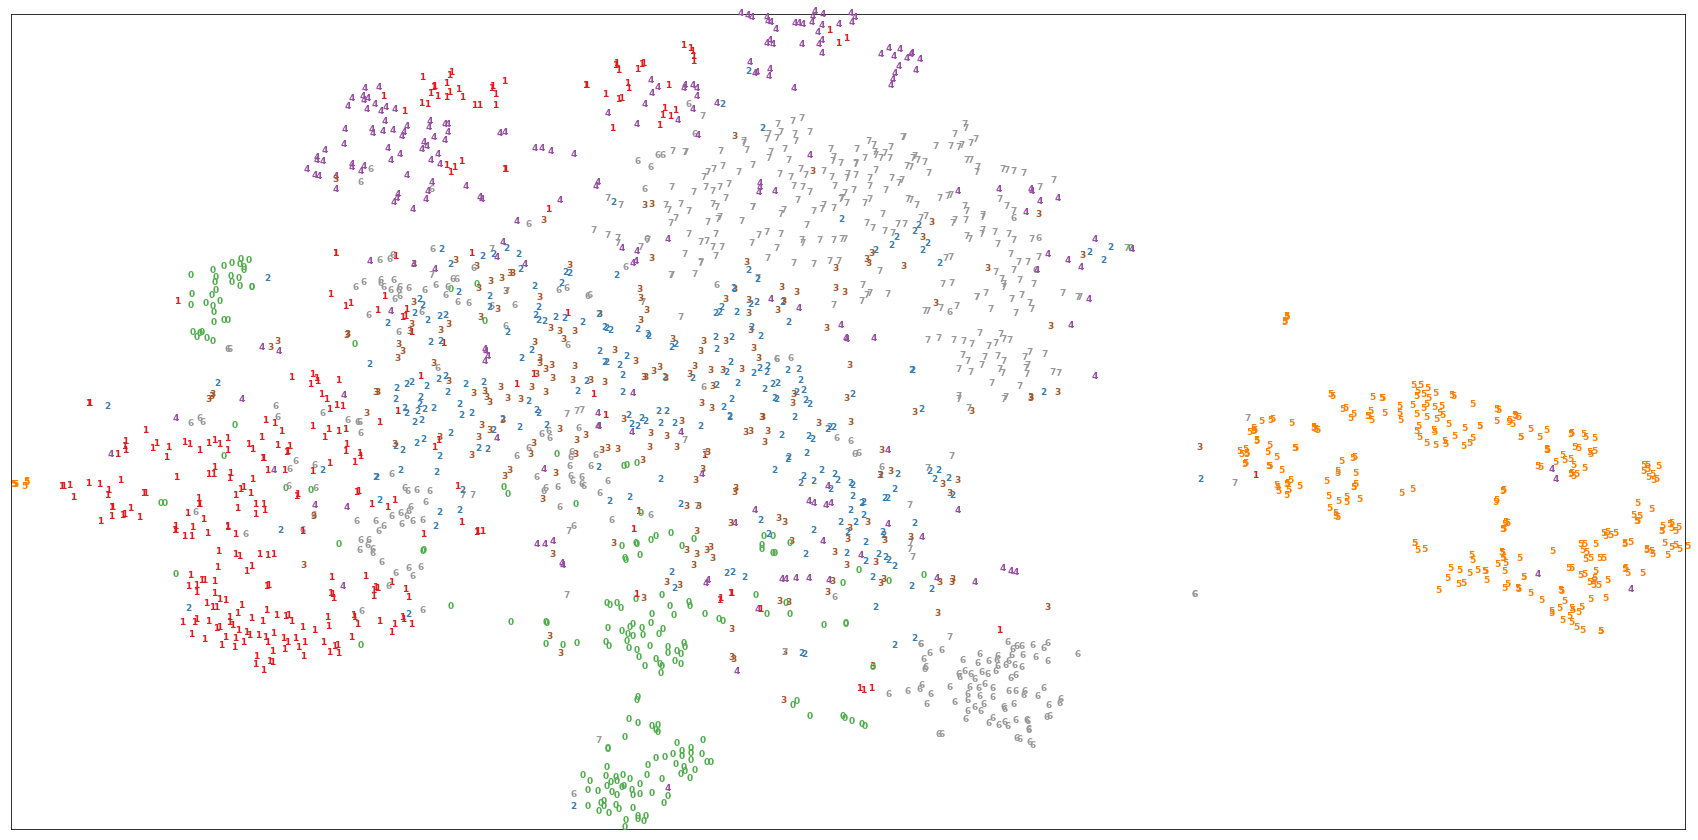
\includegraphics[width=1.0\textwidth]{img/tSNE_ReNet.png}
	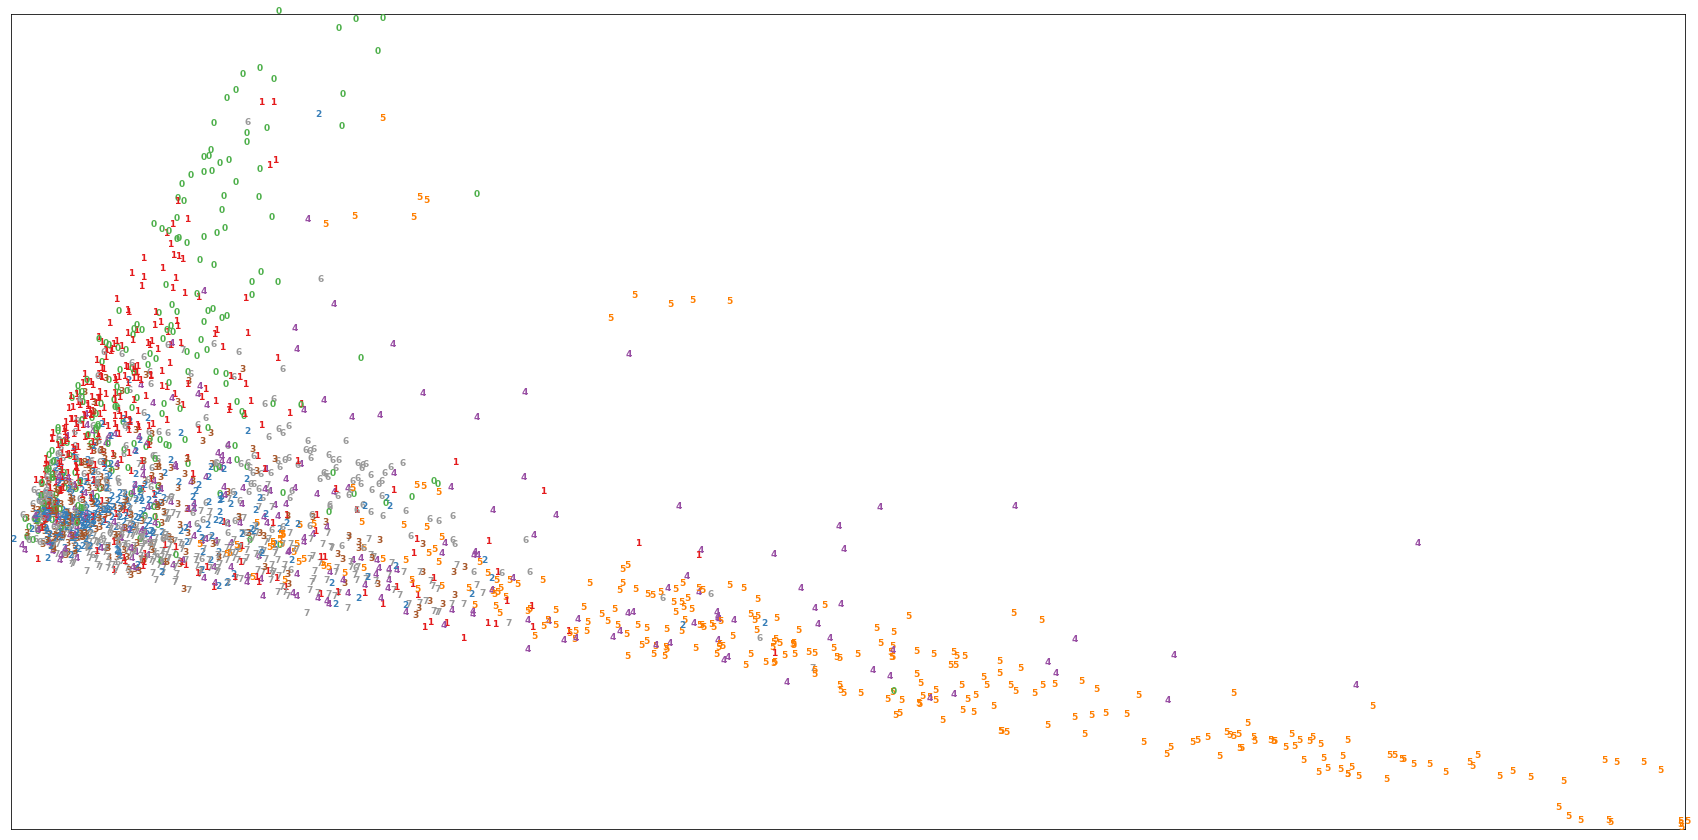
\includegraphics[width=1.0\textwidth]{img/PCA_ReNet.png}
	\caption{Wizualizacja reprezentacji nauczonej przez sieć ReNet.} (Góra) Wizualizacja wyjścia przedostatniej warstwy sieci z wykorzystaniem tSNE. (Dół) Wizualizacja wyjścia przedostatniej warstwy sieci z wykorzystaniem PCA.
	\label{fig:tSNE_ReNet}
\end{figure}

\begin{figure}
\centering
	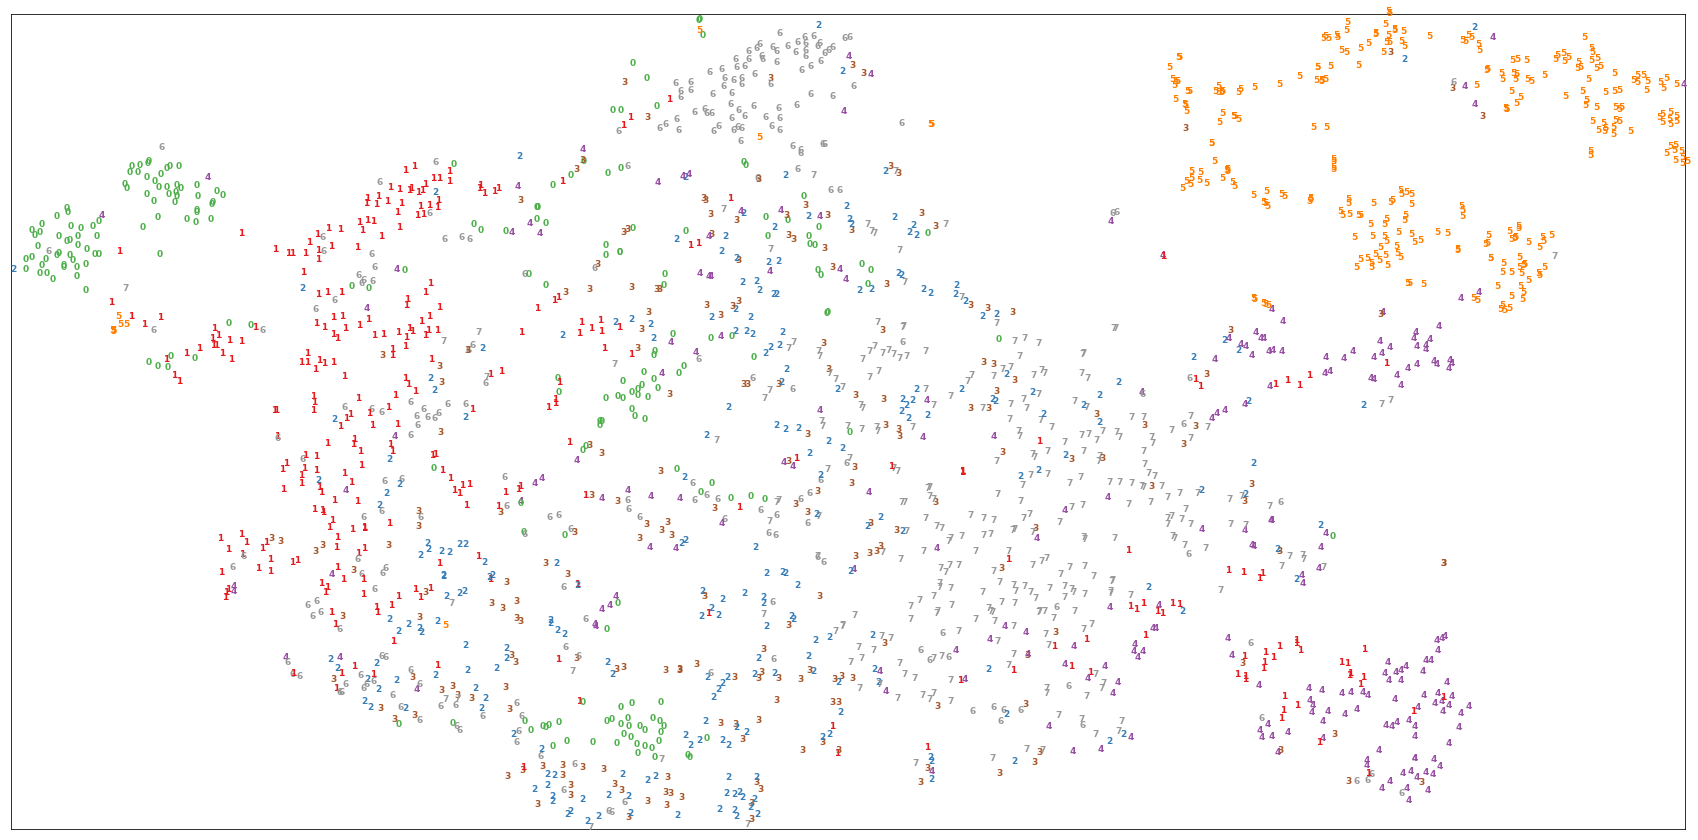
\includegraphics[width=1.0\textwidth]{img/tSNE_modif_ReNet.png}
	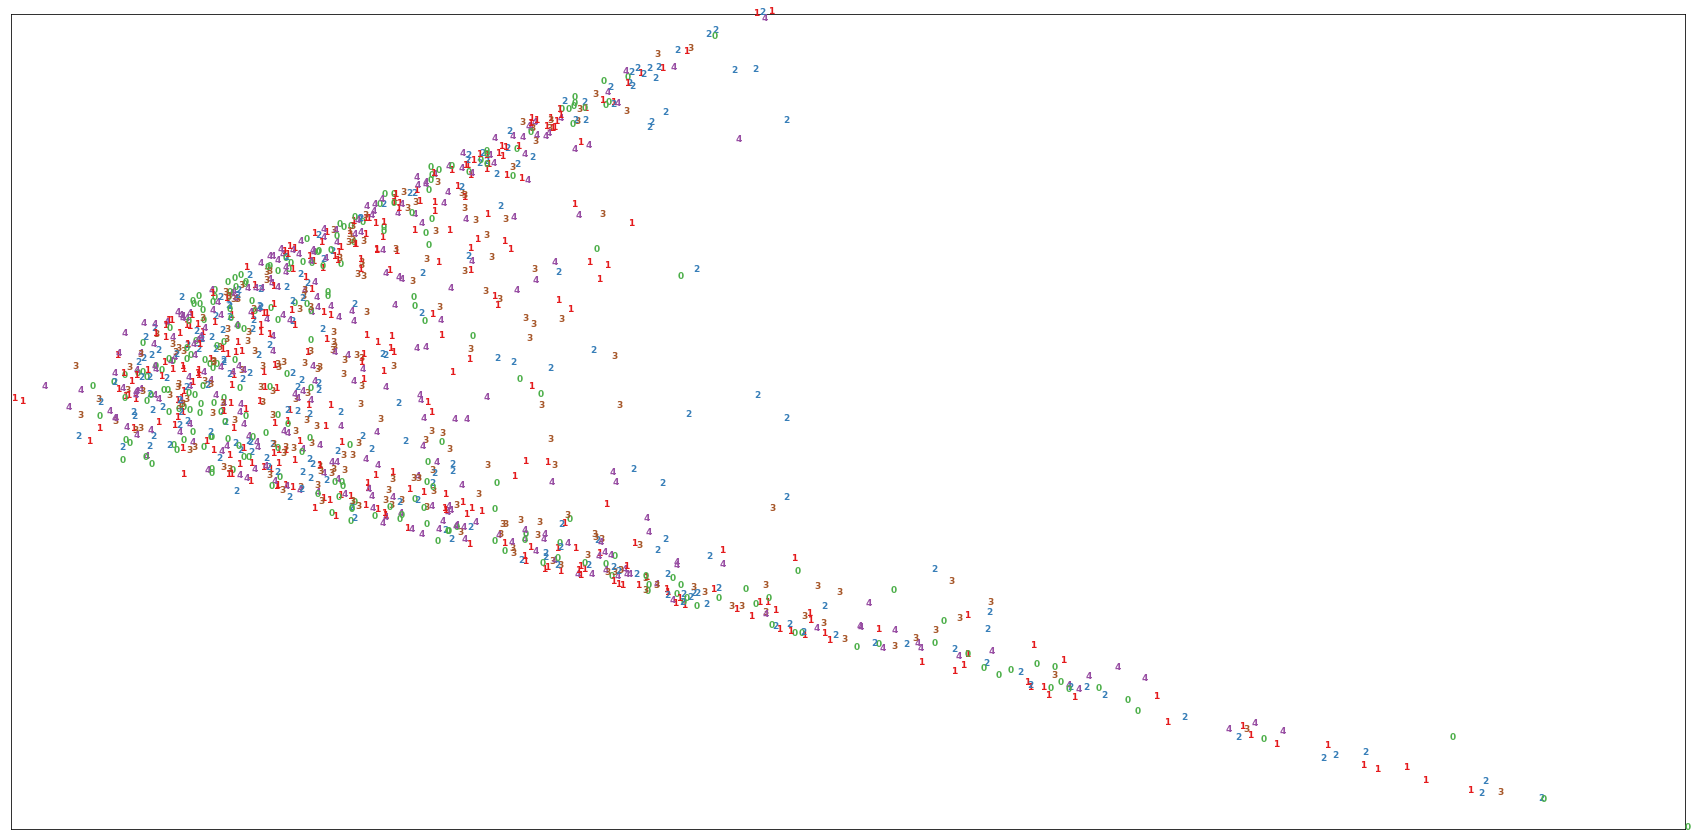
\includegraphics[width=1.0\textwidth]{img/PCA_modif_ReNet.png}
	\caption{Wizualizacja reprezentacji nauczonej przez zmodyfikowaną sieć ReNet.} (Góra) Wizualizacja wyjścia przedostatniej warstwy sieci z wykorzystaniem tSNE. (Dół) Wizualizacja wyjścia przedostatniej warstwy sieci z wykorzystaniem PCA.
	\label{fig:tSNE_modif_ReNet}
\end{figure}

\begin{figure}
\centering
	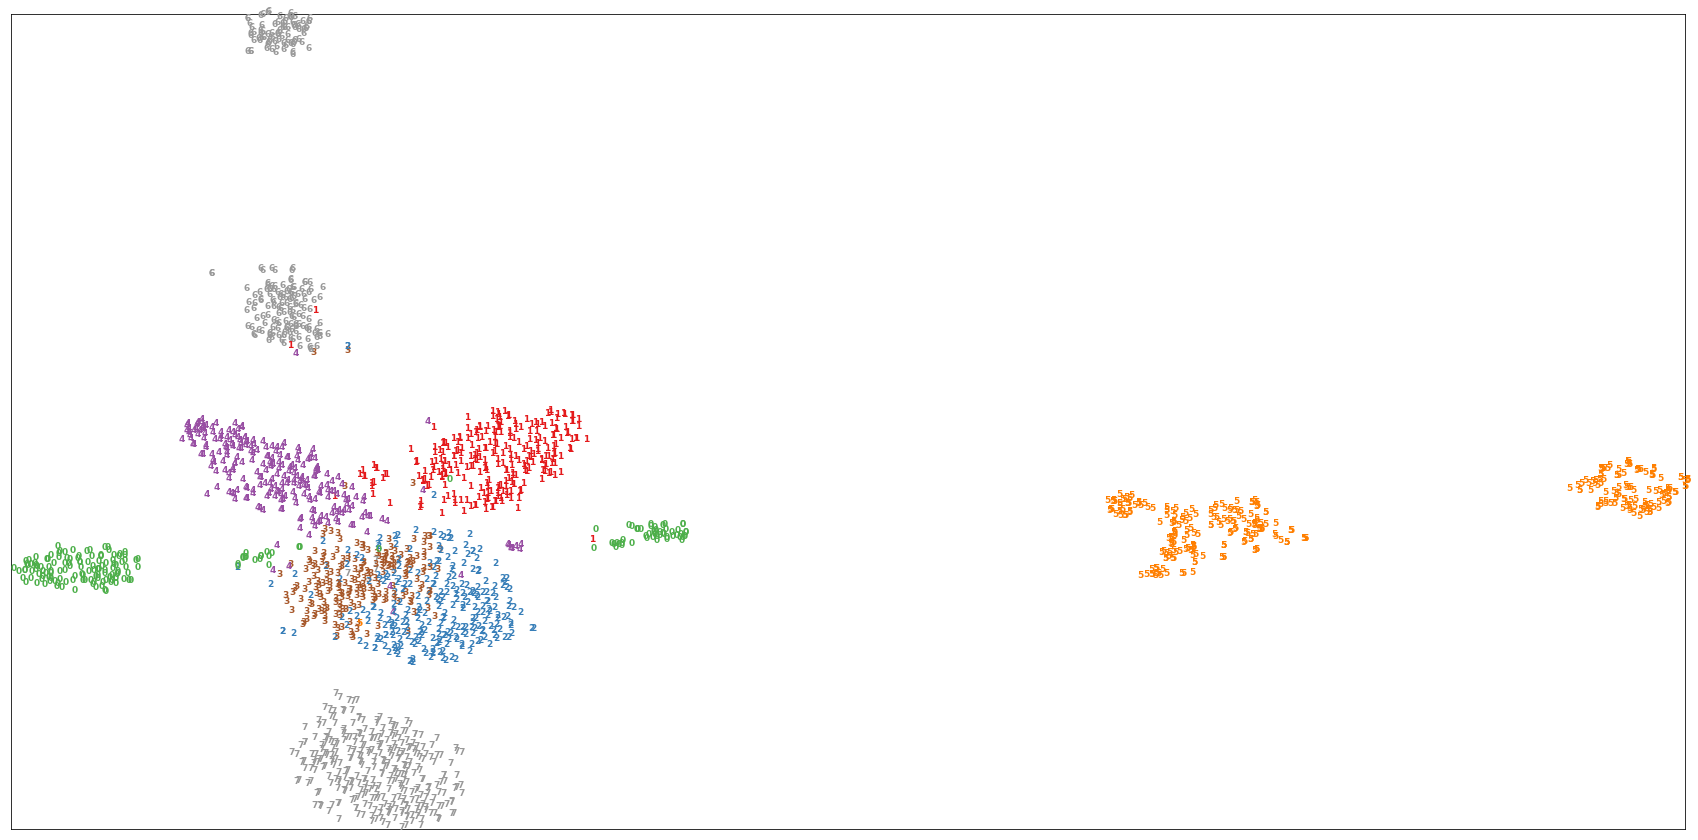
\includegraphics[width=1.0\textwidth]{img/tSNE_conv.png}
	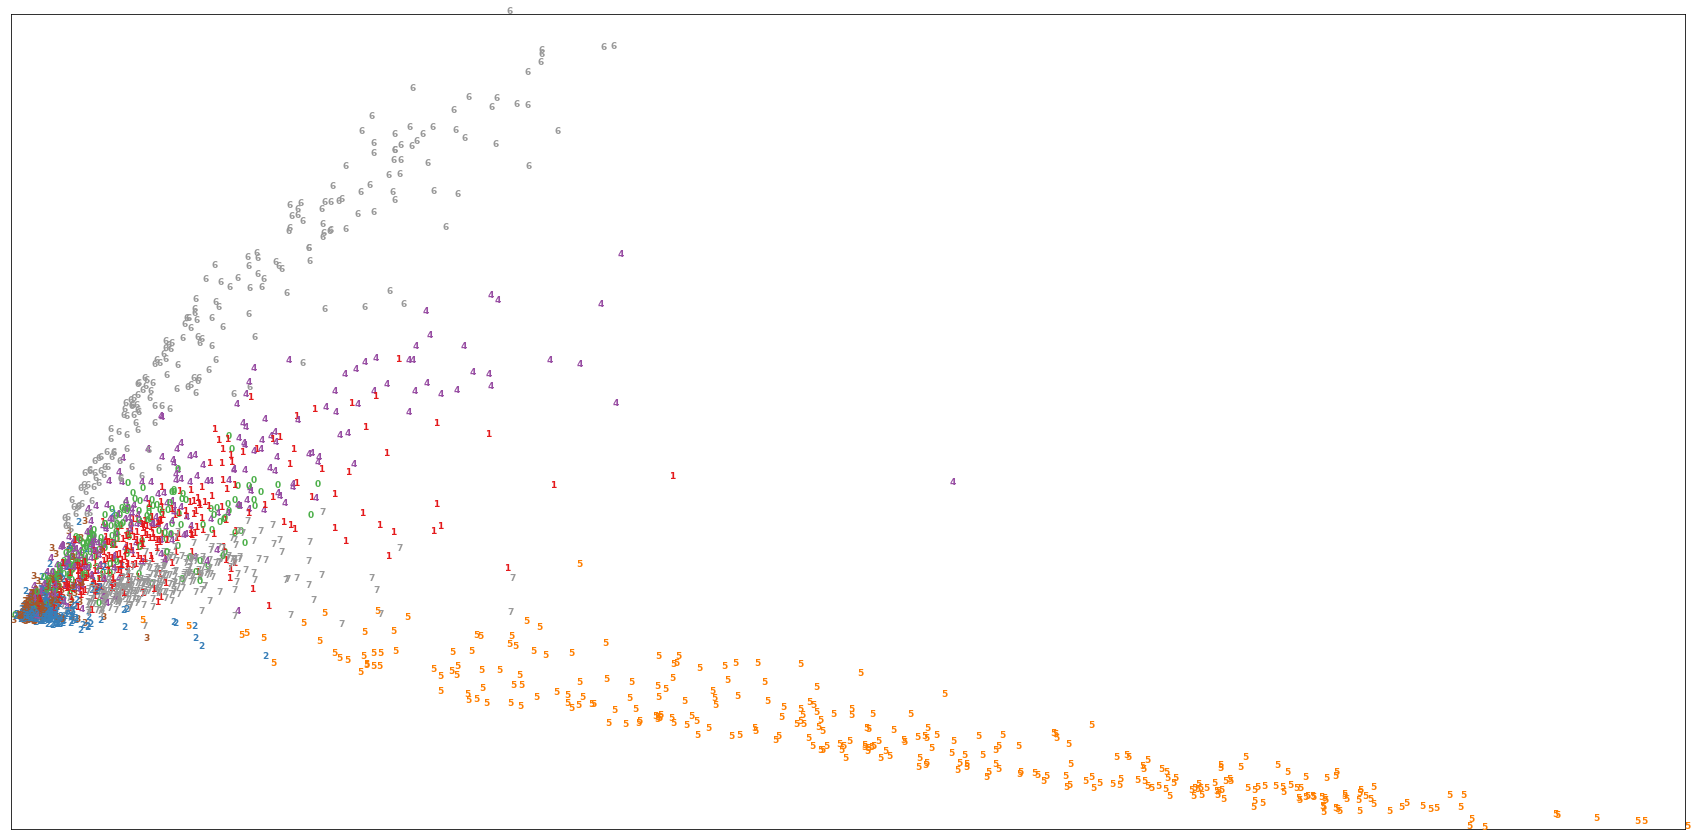
\includegraphics[width=1.0\textwidth]{img/PCA_conv.png}
	\caption{Wizualizacja reprezentacji nauczonej przez zmodyfikowaną sieć konwolucyjną.} (Góra) Wizualizacja wyjścia przedostatniej warstwy sieci z wykorzystaniem tSNE. (Dół) Wizualizacja wyjścia przedostatniej warstwy sieci z wykorzystaniem PCA.
	\label{fig:tSNE_conv}
\end{figure}

\section{Wizualizacja nauczonej reprezentacji}

W celu porównania nauczonych reprezentacji zmodyfikowanej i niezmodyfikowanej architektury ReNet przygotowano wizualizacje aktywacji przedostatniej warstwy sieci. Wektor wyjścia dla każdego przykładu ze zbioru testowego poddano redukcji wymiarowości do dwóch wymiarów. Umożliwia to przedstawienie każdego elementu zbioru testowego na płaszczyźnie i zaznaczenie klasy, do której należy przykład. Do redukcji wymiarowości wybrano algorytmy PCA i tSNE \cite{tSNE}. Wyniki dla zbioru testowego Natural Images przedstawiono na rysunkach \ref{fig:tSNE_ReNet}, \ref{fig:tSNE_modif_ReNet} i \ref{fig:tSNE_conv}.

Dla sieci konwolucyjnych przy wizualizacji t-SNE osiągnięto niemalże liniowo separowalną reprezentację. Można zaobserwować mieszanie się reprezentacji dla klas kot i pies. Bliskie położenie tych klas w przestrzeni reprezentacji jest uzasadnione biorąc pod uwagę charakter inne etykiety w datasetcie - przykładowo samochód, samolot lub kwiat. Dla sieci ReNet z uzyskanej wizualizacji wynika, że nauczona reprezentacja nie jest liniowo separowalna i wiele przykładów o różnych klasach leży blisko siebie. Istnieją pewne skupiska przykładów dla których jedna z klas dominuje, jednakże skupiska te nie są tak jednolite i zunifikowane jak w przypadku sieci konwolucyjnych.
Należy zachować szczególną ostrożność przy wyciąganiu wniosków co do geometrycznych zależności występujących w oryginalnej przestrzeni, ponieważ wizualizacje są efektem rzutowania z przestrzeni 4096-wymiarowej do przestrzeni dwuwymiarowej. Algorytm t-SNE jest skonstruowany tak aby zachowywać odległości między punktami z oryginalnej przestrzeni, jednakże nie zawsze jest w stanie oddać wszystkie niuanse występujące w oryginalnej przestrzeni. W tym przypadku geometryczna analiza nauczonej reprezentacji może podawać jedną z przyczyn słabszych wyników klasyfikacji z wykorzystaniem sieci ReNet dla datasetu Natural Images.

Zastanawiające może być przyjęcie nauczonej reprezentacji jako wyjścia przedostatniej warstwy. Dla wszystkich modeli oznacza to wykorzystanie aktywacji warstwy dropout. W czasie trenowania algorytmu mogłoby to wprowadzić losowy szum do reprezentacji. Jednakże w czasie testowania warstwa dropout skaluje jedynie każdą aktywację przez prawdopodobieństwo maskowania. Ma to na celu zachowanie średniej wartości aktywacji przekazywanych do następnej warstwy na tym samym poziomie co przy trenowaniu sieci. Wszystkie podane wizualizacje zostały wykonane w trybie testowania nauczonej sieci na zbiorze testowym, więc nie istnieje ryzyko wprowadzenia losowego szumu z powodu wybrania wyjścia dropout jako reprezentacji nauczonej przez model.

\section{Wizualizacja loss landscape}

\begin{figure}
\centering
	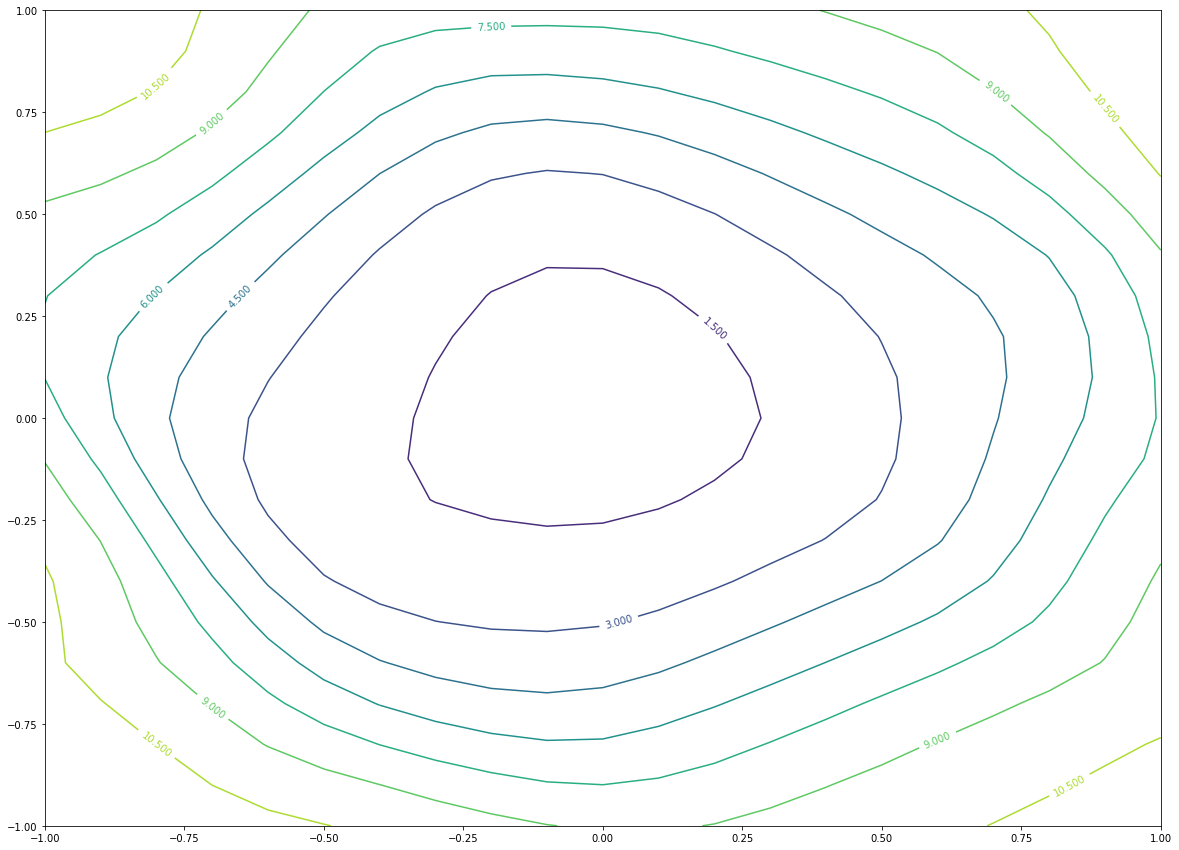
\includegraphics[width=0.49\textwidth]{img/loss_ReNet.png}
	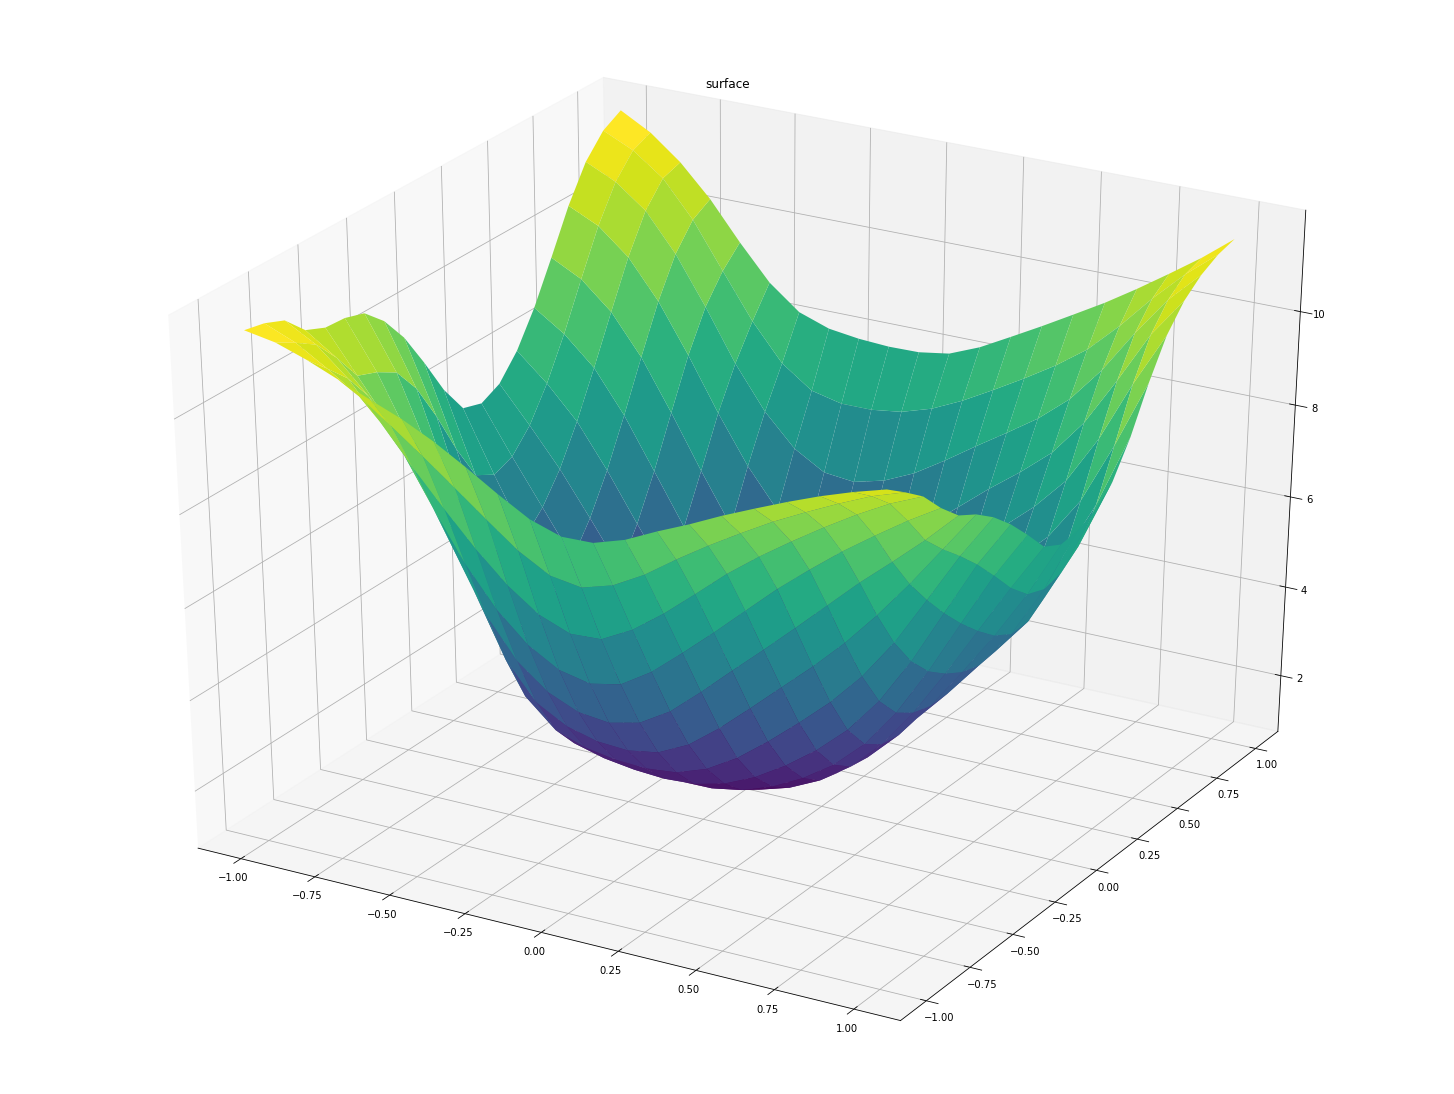
\includegraphics[width=0.49\textwidth]{img/loss_3d_ReNet.png}
	\caption{Wizualizacja loss landscape zbioru testowego nauczonej sieci ReNet.}
	\label{fig:loss_ReNet}
\end{figure}

\begin{figure}
\centering
	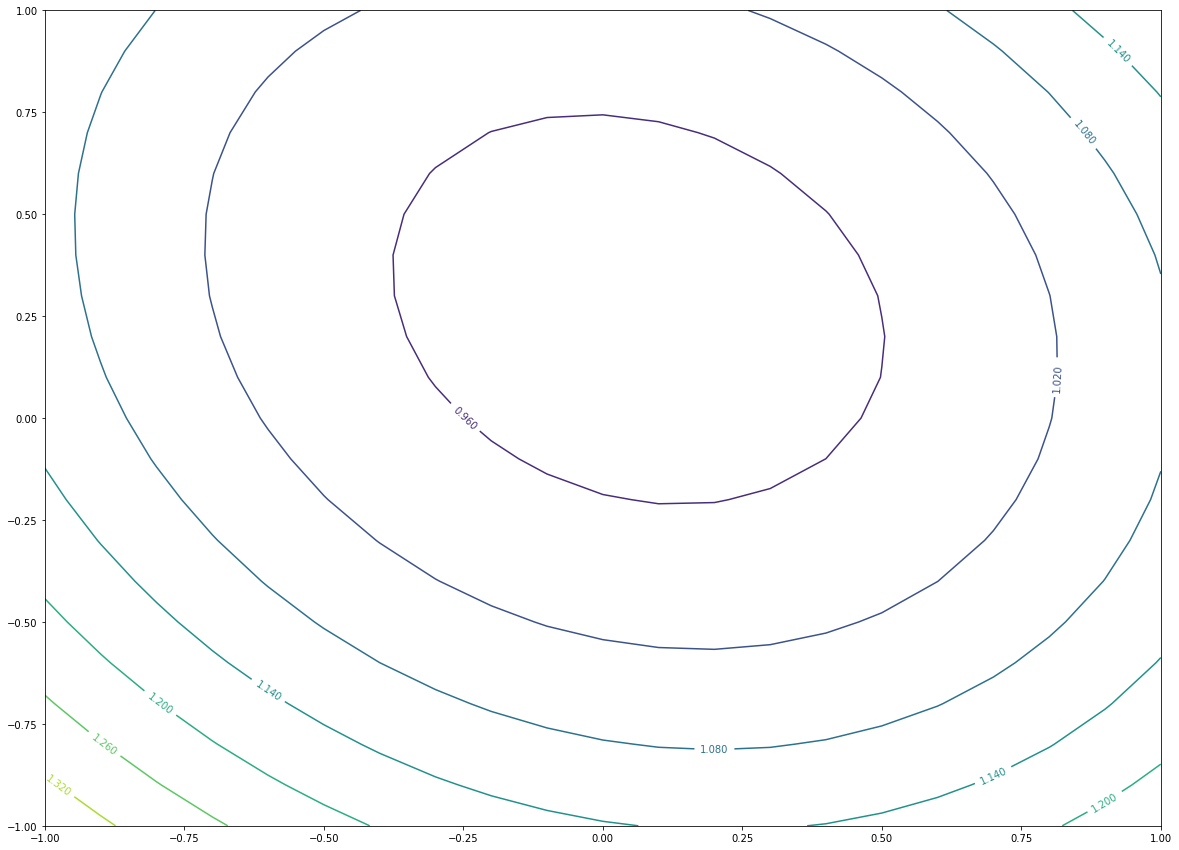
\includegraphics[width=0.49\textwidth]{img/loss_modif_ReNet.png}
	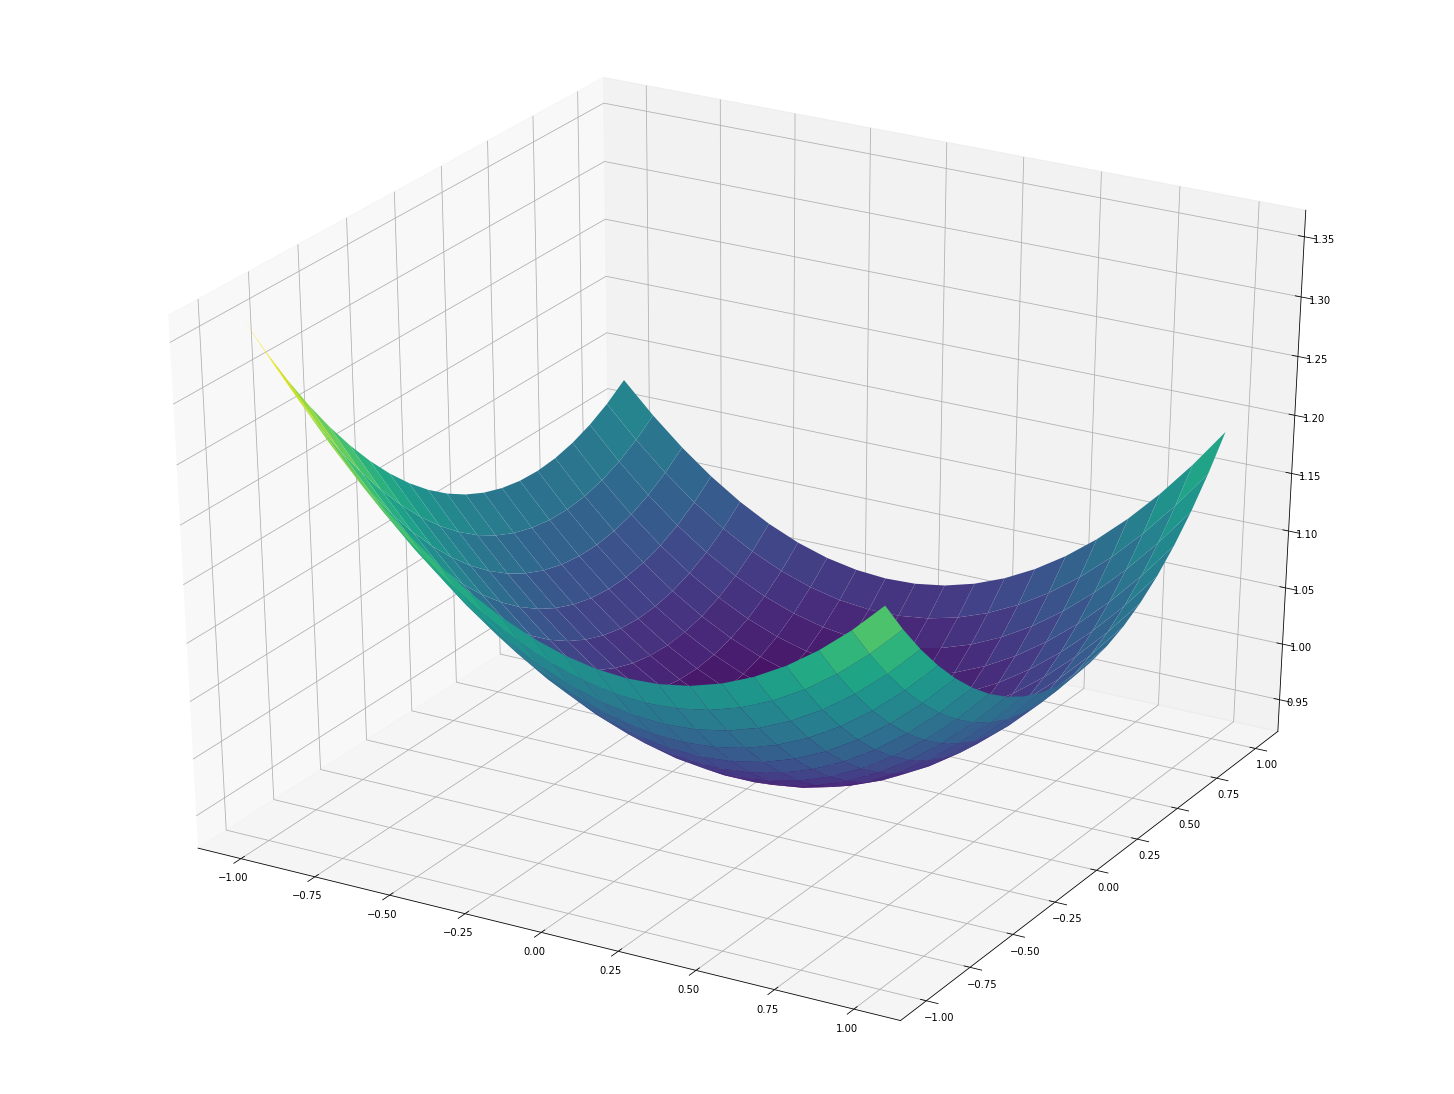
\includegraphics[width=0.49\textwidth]{img/loss_3d_modif_ReNet.png}
	\caption{Wizualizacja loss landscape zbioru testowego nauczonej zmodyfikowanej sieci ReNet.}
	\label{fig:loss_modif_ReNet}
\end{figure}

Na podstawie wizualizacji z \cite{DBLP:journals/corr/abs-1712-09913} przygotowano wizualizację loss landscape archiektur ReNet i zmodyfikowanej ReNet. Wyniki dla datasetu Flowers Recognition po 20 epokach uczeniach przedstawiono na \ref{fig:loss_ReNet} i \ref{fig:loss_modif_ReNet}. Jeśli przyjąć uzyskane wizualizacje za reprezentatywne to można zauważyć, że w obu przypadkach sieć znajduje się w minimum. Najmniejsze uzyskiwane wartości funkcji strat dla sieci ReNet były większe niż dla sieci konwolucyjnych. W przypadku w którym przyjmiemy, że osiągnięte minimum sieci jest globalne można wnioskować, że sieci ReNet nie są w stanie osiągnąć zadowalająco niskich wyników. W przypadku gdy przyjmiemy, że osiągnięte minimum nie jest globalne należy zbadać jakie metody optymalizacji byłby w stanie doprowadzić do uzyskania lepszych rezultatów. Drugi wariant jest mniej prawdopodobny ze względu na prace sugerujące, że występowanie globalnych minimum jest częstsze w płytkich sieciach neuronowych niż w głębokich, a nieglobalne minima często osiągają zbliżone wartości funkcji start do minum globalnego \cite{Goodfellow-et-al-2016}. W rozdziale tym przedstawiono i przeanalizowano wyniki uzyskane zgodnie z przyjętą metodologią. W kolejnym rozdziale zostaną przedyskutowane wnioski jakie można wyciągnąć na podstawie osiągniętych wyników.

\chapter{Wnioski}

W niniejszym rozdziale przeprowadzono dyskusję uzyskanych wyników, wskazano możliwe kierunki przyszłych badań oraz zamieszczono podziękowania dla osób, które w znaczący sposób przyczyniły się do powstania tej pracy.

\section{Podsumowanie}

Z uzyskanych wyników można wnioskować, że wprowadzenie modyfikacji zapewniło przyśpieszenie działania ReNet przy zachowaniu zbliżonej skuteczności. Umożliwia to na stosowanie głębszych modeli. Oczywiście samo stosowanie głębszych modeli nie jest zaletą samą w sobie, ale pozwala na zwiększenie elastyczności pracy z modelem. Wykorzystanie mniejszej liczby sieci LSTM na warstwę ReNet umożliwia bardziej precyzyjnie dobranie liczby stosowanych warstw ReNet do rozwiązywanego problemu. Tym samym wyniki potwierdziły przypuszczenia ze wstępu pracy i z wprowadzenia teoretycznych podstaw modyfikacji ReNet.

Na zakończenie pracy można zastanowić się czy wprowadzone usprawnienia są wystarczające aby ReNet zyskało na praktycznym znaczeniu? Wyniki wskazują na to, że nie jest to prawdopodobne. Mimo redukcji czasu uczenia nadal wymagane są znaczące nakłady mocy obliczeniowej, a osiągane wyniki są gorsze niż dla sieci konwolucyjnych. Zastosowane wizualizacje wskazują dodatkowe potencjalne przyczyny osiągania gorszych wyników sieci ReNet. Wymagane są dalsze usprawnienia w zakresie poprawy osiągów i wydajności. 

Jednym z możliwych powodów wydłużonego czasu uczenia sieci rekurencyjnych może być ich struktura grafu obliczeniowego. Jest on sekwencyjny, co przekłada się na sposób przeprowadzania obliczeń i możliwe optymalizacje. Obecny sprzęt wykorzystywany do obliczeń przy głębokich sieciach neuronowych jest przystosowany do wykonywania wielu prostych i powtarzających obliczeń jednocześnie, co doskonale sprawdza się w przypadku sieci konwolucyjnych. Dla obliczeń z sekwencyjnym grafem zależności takim jak dla sieci rekurencyjnych wykonanie obliczeń dla danego kroku czasowego może nastąpić po wyznaczeniu potrzebnych wartości z poprzedniego kroku czasowego, co może powodować częstsze korzystanie z pamięci oraz wydłużenie czasu obliczeń. Dlatego momentami możliwe jest szybsze nauczenie małej sieci rekurencyjnej na CPU niż na GPU. 

Przez duże koszty obliczeniowe zakres zastosowań ReNet jest ograniczony do obrazów o małym rozmiarze. Ograniczenia te redukują liczbę cech dostępnych na wejściu sieci tym samym utrudniają uczenie. Mimo zastosowania tych ograniczeń sieci konwolucyjne nadal radzą sobie lepiej z uczeniem datasetów przedstawionych w tej pracy. Możliwe jest wykorzystanie sieci residualnych do zadań machine vision, jednakże nie było potrzeby stosowania tak skomplikowanych modeli w tej pracy.

\section{Możliwe usprawnienia i dalsze kierunki badań}

Dalsze badania w zakresie sieci ReNet mogą obejmować zbadanie zastosowania tej architektury do zbiorów zawierających dużo klas i mało przykładów uczących na klasę. W trakcie pracy odnotowano, że stosowane modele osiągają skuteczność na poziome klasyfikatora losowego, podczas gdy sieci konwolucyjne na tych samych danych osiągały wyższą skuteczność. Ciekawym eksperymentem może być zredukowanie rozmiaru patrzy do rozmiaru pojedynczego piksela i zastosowanie warstw Batch Normalisation. Dodatkowo można zbadać jak zachowa się sieć ReNet przy stosowaniu zwiększającej się liczby neurownów w kolejnych warstwach, tak jak ma to miejsce w sieciach konwolucyjnych.

W przypadku zmodyfikowanej sieci ReNet właściowści krzywej Hilberta mogą pozwolić na zmianę rozmiarów obrazów i sprawdzenia jak sieć nauczona dla mniejszych obrazów poradzi sobie z większymi obrazami. Tego typu manipulacje są ograniczone przez ścisłe wymagania odnośnie struktury sieci i kształtu tensorów, ale można je obejść przez zastosowanie dodatkowej warstwy ReNet lub MaxPooling.

W początkowym projekcie eksperymentu zakładano przeprowadzenie badań wpływu zastosowanej sieci rekurencyjnej na wyniki klasyfikacji ReNet z modyfikacją. Jednakże ograniczenia czasowe nie pozwoliły na zrealizowanie tego celu i pozostaje on otwartym problemem badawczym.

\bibliography{bibliography}

\listoffigures

\end{document}